\documentclass[11pt,a4paper,ngerman]{report}
% sostituire con report/book per il formato elettronico

\usepackage[nottoc,notlof,notbib,notindex]{tocbibind} % include l'elenco delle figure e la bibliografia nell'indice.
\usepackage{url}
\usepackage{pdfpages}
\usepackage{tocloft}
\usepackage{appendix}
\usepackage{tabularx, caption, boldline}
\usepackage{array}
%\usepackage{multirow}
\usepackage[ngerman, english]{babel}
\usepackage{ucs} %unicode sistema gli accenti
\usepackage[utf8]{inputenc} %unicode sistema gli accenti utf8x
\usepackage{csquotes}
\usepackage[bottom]{footmisc} % posiziona le note in footer sempre in basso
\usepackage{fancyhdr}
\usepackage{graphicx}
\usepackage{color}
%\usepackage{subfigure} % per figure affiancate
\usepackage{subcaption}
\usepackage{supertabular} % used to break tables
\usepackage{float} % per far bene le figures
%\usepackage{indentfirst}
\usepackage[Lenny]{fncychap} % per cambiare i capitoli
\usepackage{longtable} % piazza le note nelle tabelle fuori dalla tabella e permette tabelle che spannano su più pagine
\usepackage{lastpage} % total page count
\usepackage[hyphens]{url}
%\usepackage{breakurl}
\usepackage{tikz}
\usepackage{verbatim}
\usepackage{amsmath}
\usepackage{amssymb}
\usepackage{comment}
\usepackage[colorlinks=true, pdfstartview=FitV, linkcolor=blue, citecolor=blue, urlcolor=blue,breaklinks=true]{hyperref}
\usepackage{listings}
\usepackage{xcolor}
\usepackage{booktabs}
\usepackage{wrapfig}

\usepackage[T1]{fontenc}
\usepackage{inconsolata}


\definecolor{pblue}{rgb}{0.13,0.13,1}
\definecolor{pgreen}{rgb}{0,0.5,0}
\definecolor{pred}{rgb}{0.9,0,0}
\definecolor{pgrey}{rgb}{0.46,0.45,0.48}


% colori e variabili
% color definitions
\definecolor{red}{rgb}{0.9,0.1,0.1}
\definecolor{blue}{rgb}{0.07,0.55,0.73}
\definecolor{purple}{rgb}{0.4,0.3,0.4}
\definecolor{deep}{rgb}{0.1,0.07,0.3}
\definecolor{white}{rgb}{0.9,0.8,0.86}
% per modificare il colore dei link andare su layout.tex
%layout legacy commands
\renewcommand{\sectionmark}[1]{\markright{\thesection.\ #1}}
\renewcommand{\chaptermark}[1]{\markboth{\thechapter.\ #1}{}}

%user defined commands

% defnisce una pagina bianca con stile plain (migliore delle pagine bianche inserite in automatico dal model book)
\newcommand{\blankpage}{
	\newpage
	% toglie la barra alta dalla pagina vuota
	\thispagestyle{plain}
	% forza una pagina vuota
	\mbox{}
	\newpage
}

%comando per inserire la premessa nel documento (fuori indice)
\newcommand{\premise}[1][]{
	\renewcommand{\theenumi}{#1\roman{enumi}}
	\renewcommand{\labelenumi}{(\theenumi)}
	\thispagestyle{plain}
}


%comandi creati per le convenzioni del documento:
\newcommand{\istage}{\textit{stage}}
\newcommand{\iStage}{\textit{Stage}}
\newcommand{\idfda}{\textit{D.F.D. Assessment System}}
\newcommand{\idfd}{\textit{D.F.D. Consulting}}
\newcommand{\iIT}{\textit{IT}}
\newcommand{\iICT}{\textit{ICT}}
\newcommand{\ibusiness}{\textit{business}}





% indice analitico (comandi con la 'i' scrivono e aggiungono, quelli con 'ii' aggiungono solo, quelli senza niente scrivono solo)
\newcommand{\iASI}{ASI\index{ASI}} %scrive C sharp

%tecnologie
\newcommand{\CSharp}{C♯} %scrive C sharp
\newcommand{\iCSharp}{C♯\index{C♯}} % scrive C sharp e aggiunge l'indice %\unichar{9839}
\newcommand{\idotNET}{.NET\index{.NET}} % scrive .NEt e aggiunge l'indice
\newcommand{\iiWPF}{\index{WPF}} % aggiunge solo l'indice a WPF
\newcommand{\iWPF}{WPF\index{WPF}} % scrive WPF e aggiunge l'indice
\newcommand{\iiWF}{\index{WinForms}}
\newcommand{\iAW}{ANTLRWorks\index{ANTLRWorks}}
\newcommand{\iA}{ANTLR\index{ANTLR}}
\newcommand{\iU}{Unicode\index{Unicode}}
\newcommand{\iPSharp}{\texttt{PdfSharp}\index{PdfSharp@\texttt{PdfSharp}}}
\newcommand{\iTSharp}{\texttt{iTextSharp}\index{iTextSharp@\texttt{iTextSharp}}}

%grammatica
\newcommand{\iiCFG}{\index{CFG (context-free grammar)}}

%programmi
\newcommand{\iVS}{Visual Studio\index{Visual Studio}}
\newcommand{\iVSS}{Visual SourceSafe\index{Visual SourceSafe}}
\newcommand{\iSS}{SQL Server\index{SQL Server}}

% ciclo attivo e passivo
\newcommand{\iCA}{ciclo attivo\index{ciclo!attivo}} % scrive ciclo attivo e aggiunge l'indice
\newcommand{\iCP}{ciclo passivo\index{ciclo!passivo}} % scrive ciclo passivo e aggiunge l'indice
\newcommand{\iiCA}{\index{ciclo!attivo}} % aggiunge l'indice
\newcommand{\iiCP}{\index{ciclo!passivo}} % aggiunge l'indice
\newcommand{\iDCA}{ciclo attivo\index{documento!ciclo attivo}} % scrive ciclo attivo agigunge l'indice al ciclo attivo del documento
\newcommand{\iDCP}{ciclo passivo\index{documento!ciclo passivo}} % scrive ciclo passivo aggiunge l'indice al ciclo passivo del documento
\newcommand{\iiDCA}{\index{documento!ciclo attivo}} % aggiunge l'indice al ciclo attivo del documento
\newcommand{\iiDCP}{\index{documento!ciclo passivo}} % aggiunge l'indice al ciclo passivo del documento
\newcommand{\iGCA}{ciclo attivo\index{gestione!ciclo attivo}} % scrive ciclo attivo e aggiunge l'indice a gestione
\newcommand{\iGCP}{ciclo passivo\index{gestione!ciclo passivo}} % scrive ciclo passivo e aggiunge l'indice a gestione
\newcommand{\iiGCP}{\index{gestione!ciclo passivo}} % aggiunge l'indice a gestione

%componenti
\newcommand{\icMM}{\texttt{MapManager}\index{MapManager@\texttt{MapManager}}}
\newcommand{\iicMM}{\index{MapManager@\texttt{MapManager}}}
\newcommand{\icMF}{\texttt{MapFinder}\index{MapFinder@\texttt{MapFinder}}}
\newcommand{\iicMF}{\index{MapFinder@\texttt{MapFinder}}}
\newcommand{\icPA}{\texttt{PdfAnalyzer}\index{PdfAnalyzer (componente)@\texttt{PdfAnalyzer} (componente)}}

%package e classi
\newcommand{\iPFE}{\texttt{Plain.File.Extraction}\index{Plain.File.Extraction@\texttt{Plain.File.Extraction}}}
\newcommand{\iiPFE}{\index{Plain.File.Extraction@\texttt{Plain.File.Extraction}}}
\newcommand{\iPA}{\texttt{PdfAnalyzer}\index{Plain.File.Extraction@\texttt{Plain.File.Extraction}!PdfAnalyzer (classe)@\texttt{PdfAnalyzer} (classe)}}
\newcommand{\iPP}{\texttt{PdfPage}\index{Plain.File.Extraction@\texttt{Plain.File.Extraction}!PdfPage@\texttt{PdfPage}}}
\newcommand{\iPPar}{\texttt{PdfTextStreamParser}\index{Plain.File.Extraction@\texttt{Plain.File.Extraction}!PdfTextStreamParser@\texttt{PdfTextStreamParser}}}
\newcommand{\iPLex}{\texttt{PdfTextStreamLexer}\index{Plain.File.Extraction@\texttt{Plain.File.Extraction}!PdfTextStreamLexer@\texttt{PdfTextStreamLexer}}}
\newcommand{\iPF}{\texttt{PdfFont}\index{Plain.File.Extraction@\texttt{Plain.File.Extraction}!PdfFont@\texttt{PdfFont}}}
\newcommand{\iPT}{\texttt{PdfText}\index{Plain.File.Extraction@\texttt{Plain.File.Extraction}!PdfText@\texttt{PdfText}}}
\newcommand{\iPC}{\texttt{PdfChar}\index{Plain.File.Extraction@\texttt{Plain.File.Extraction}!PdfChar@\texttt{PdfChar}}}

%parti di un PDF
\newcommand{\iH}{\texttt{Header}\index{PDF!Header@\texttt{Header}}}
\newcommand{\iFT}{\texttt{File Trailer}\index{PDF!File Trailer@\texttt{File Trailer}}}
\newcommand{\iCRTable}{\texttt{Cross Reference Table}\index{PDF!Cross Reference Table@\texttt{Cross Reference Table}}}
\newcommand{\iB}{\texttt{Body}\index{PDF!Body@\texttt{Body}}}

% stream
\newcommand{\iS}{stream\index{stream}}
\newcommand{\iiS}{\index{stream}}
\newcommand{\iCS}{stream\index{content stream}}
\newcommand{\iiCS}{\index{content stream}}

%fasi dello stage
\newcommand{\iifS}{\index{studio del dominio!fase di}}
\newcommand{\iifA}{\index{analisi!fase di}}
\newcommand{\iifP}{\index{progettazione!fase di}}
\newcommand{\iifC}{\index{codifica!fase di}}
\newcommand{\iifV}{\index{verifica e validazione!fase di}}
\newcommand{\iifD}{\index{documentazione!fase di}}

%attività dello stage
\newcommand{\iiaS}{\index{studio del dominio!attività di}}
\newcommand{\iiaA}{\index{analisi!attività di}}
\newcommand{\iiaP}{\index{progettazione!attività di}}
\newcommand{\iiaC}{\index{codifica!attività di}}
\newcommand{\iiaV}{\index{verifica e validazione!attività di}}
\newcommand{\iiaD}{\index{documentazione!attività di}}

%matrici
\newcommand{\Tm}{$T_{m}$}
\newcommand{\Tlm}{$T_{lm}$}

%peratori
\newcommand{\Tc}{\texttt{Tc}\index{operatore!di stato}}
\newcommand{\Tw}{\texttt{Tw}\index{operatore!di stato}}
\newcommand{\Tz}{\texttt{Tz}\index{operatore!di stato}}
\newcommand{\TL}{\texttt{TL}\index{operatore!di stato}}
\newcommand{\Tf}{\texttt{Tf}\index{operatore!di stato}}
\newcommand{\Tr}{\texttt{Tr}\index{operatore!di stato}}
\newcommand{\Ts}{\texttt{Ts}\index{operatore!di stato}}

\newcommand{\Td}{\texttt{Td}\index{operatore!di posizionamento}}
\newcommand{\Tmm}{\texttt{Tm}\index{operatore!di posizionamento}}
\newcommand{\Tstar}{\texttt{T*}\index{operatore!di posizionamento}}

\newcommand{\Tj}{\texttt{Tj}\index{operatore!di stampa}}
\newcommand{\Tquote}{\texttt{'}\index{operatore!di stampa}}
\newcommand{\Tdblquote}{\texttt{\textquotedbl}\index{operatore!di stampa}}
\newcommand{\TJ}{\texttt{TJ}\index{operatore!di stampa}}










\graphicspath{{./pics/}} % cartella di salvataggio immagini

\pagestyle{fancy}

\lhead{\nouppercase{\rightmark}}
\rhead{\nouppercase{\leftmark}}

\fancypagestyle{plain}{
	\lhead{}
	\chead{}
	\rhead{}
	\lfoot{}
	\cfoot{\thepage}
	\rfoot{}
	\renewcommand{\headrulewidth}{0.0pt}% this command should not be add to variables.tex
	\renewcommand{\footrulewidth}{0.1pt}% this command should not be add to variables.tex
}

\fancypagestyle{blank}{
	\lhead{}
	\chead{}
	\rhead{\nouppercase{\rightmark}}
	\lfoot{}
	\cfoot{\thepage}
	\rfoot{}
	\renewcommand{\headrulewidth}{0.1pt}% this command should not be add to variables.tex
	\renewcommand{\footrulewidth}{0.1pt}% this command should not be add to variables.tex
}



% parte per il report
 %	\lhead{}
% 	\chead{}
% 	\rhead{\nouppercase{\rightmark}}
% 	\lfoot{}
% 	\cfoot{\thepage}
% 	\rfoot{}
% 	\renewcommand{\headrulewidth}{0.1pt}% this command should not be add to variables.tex
% 	\renewcommand{\footrulewidth}{0.1pt}% this command should not be add to variables.tex
 
 %\hypersetup{
 %	colorlinks=true,% false: boxed links; true: colored links
% 	linkcolor=blue,% color of internal links
% 	urlcolor=blue,% color of external links
% 	anchorcolor = blue,
% 	citecolor = blue
 %}
%parte per il report



% parte per il book
\fancyhead{}
%\fancyhead[EL]{\nouppercase{\leftmark}}
\fancyhead[OR]{\nouppercase{\rightmark}}
%\fancyfoot[EC,OC]{\thepage}

	\renewcommand{\headrulewidth}{0.1pt}% this command should not be add to variables.tex
	\renewcommand{\footrulewidth}{0.1pt}% this command should not be add to variables.tex
\hypersetup{
	colorlinks=true,% false: boxed links; true: colored links
	linkcolor=black,% color of internal links
	urlcolor=black,% color of external links
	anchorcolor = black,
	citecolor = black
}
%parte per il book
\newcommand{\changelocaltocdepth}[1]{%
	\addtocontents{toc}{\protect\setcounter{tocdepth}{#1}}%
	\setcounter{tocdepth}{#1}%
}

\setlength{\parindent}{0pt}

% indice analitico
\usepackage{makeidx}
\makeindex 

\let\textquotedbl=" % use to print also " in the code


\bibliographystyle{plain}%bibliografia stile inglese

\pagenumbering{Roman}
% fine layout

\newcommand{\figuresource}[1]{\small \par Quelle: #1}

\colorlet{punct}{red!60!black}
\definecolor{background}{HTML}{EEEEEE}
\definecolor{delim}{RGB}{20,105,176}
\colorlet{numb}{magenta!60!black}

\definecolor{pblue}{rgb}{0.13,0.13,1}
\definecolor{pgreen}{rgb}{0,0.5,0}
\definecolor{pred}{rgb}{0.9,0,0}
\definecolor{pgrey}{rgb}{0.46,0.45,0.48}

\lstset{language=Java,
  basicstyle=\footnotesize=7\ttfamily,
  morekeywords={@NotNull},
  numbers=left,
  stepnumber=1,
  showspaces=false,
  frame=lines,
  showtabs=false,
  breaklines=true,
  showstringspaces=false,
  breakatwhitespace=true,
  commentstyle=\color{pgreen},
  backgroundcolor=\color{background},
  keywordstyle=\color{pblue},
  stringstyle=\color{pred},
  moredelim=[il][\textcolor{pgrey}]{$$},
  moredelim=[is][\textcolor{pgrey}]{\%\%}{\%\%}
}

\lstdefinelanguage{json}{
	basicstyle=\normalfont\ttfamily,
	numbers=left,
	numberstyle=\scriptsize,
	stepnumber=1,
	showstringspaces=false,
	breaklines=true,
	frame=lines,
	backgroundcolor=\color{background},
	literate=
	{0}{{{\color{numb}0}}}{1}
	{1}{{{\color{numb}1}}}{1}
	{2}{{{\color{numb}2}}}{1}
	{3}{{{\color{numb}3}}}{1}
	{4}{{{\color{numb}4}}}{1}
	{5}{{{\color{numb}5}}}{1}
	{6}{{{\color{numb}6}}}{1}
	{7}{{{\color{numb}7}}}{1}
	{8}{{{\color{numb}8}}}{1}
	{9}{{{\color{numb}9}}}{1}
	{:}{{{\color{punct}{:}}}}{1}
	{,}{{{\color{punct}{,}}}}{1}
	{\{}{{{\color{delim}{\{}}}}{1}
	{\}}{{{\color{delim}{\}}}}}{1}
	{[}{{{\color{delim}{[}}}}{1}
	{]}{{{\color{delim}{]}}}}{1},
}

\lstdefinelanguage{SQL}{
	basicstyle=\normalfont\ttfamily,
	numbers=left,
	numberstyle=\scriptsize,
	stepnumber=1,
	numbersep=8pt,
	showstringspaces=false,
	breaklines=true,
	frame=lines,
	backgroundcolor=\color{background},
	literate=
	{0}{{{\color{numb}0}}}{1}
	{1}{{{\color{numb}1}}}{1}
	{2}{{{\color{numb}2}}}{1}
	{3}{{{\color{numb}3}}}{1}
	{4}{{{\color{numb}4}}}{1}
	{5}{{{\color{numb}5}}}{1}
	{6}{{{\color{numb}6}}}{1}
	{7}{{{\color{numb}7}}}{1}
	{8}{{{\color{numb}8}}}{1}
	{9}{{{\color{numb}9}}}{1}
	{:}{{{\color{punct}{:}}}}{1}
	{,}{{{\color{punct}{,}}}}{1}
	{\{}{{{\color{delim}{\{}}}}{1}
	{\}}{{{\color{delim}{\}}}}}{1}
	{[}{{{\color{delim}{[}}}}{1}
	{]}{{{\color{delim}{]}}}}{1},
}

\newcommand{\TODO}[1]{\marginpar{\color{red}\emph{\small{{\bf TODO: } #1}}}}
% layout
\begin{document}
\hyphenation{
Plugin-Arch-it-ekt-ur
}


%word division
% Frontespizio
\begin{titlepage}
\begin{center}
	\vspace{6em}
	{\Large \textsc{Projektbericht}}\\
	\vspace{5em}
	{\huge \textsc{Hamaube}}\\
	\vspace{4em}
	{\Large \textsc{Kai Martinen, Fabian Kohler, Merlin Koglin, Arkadij Daschkewitsch, Rasmus Warrelmann, David Zschocke }}\\
	\vspace{3em}
	{\Large \textsc{\today}}\\
	\vspace{3em}
	
\includegraphics[scale=0.4]{uni-logo.jpg}\\
	\vspace{3em}
	{\Large \textsc{Universität Hamburg}}\\
	\vspace{1em}
	{\Large \textsc{Department of Computer Science}}\\
	\vspace{1em}
	{\Large \textsc{Chair of Distributed Systems and Information Systems}}\\
	\vspace{2em}
	{\Large \textsc{Betreut durch Steffen Friedrich}}\\
	
\end{center}
\end{titlepage}%for the cover title

%If want to write a dedication, modify the following.
%\dedication{Zitat, kluger Spruch oder Widmung}

\newcommand{\TODO}[1]{\marginpar{\color{red}\emph{\small{{\bf TODO: } #1}}}}

\newpage
\chapter*{Abstract}
\addcontentsline{toc}{chapter}{Abstract}
Abstract in English

\chapter*{Kurzfassung}
\addcontentsline{toc}{chapter}{Kurzfassung} 
Kurzfassung auf Deutsch



% Old Abstract
%\newpage
%\blankpage
%\premise{
%\noindent{\textbf{\begin{huge}Abstract\end{huge}}}\\
%\\
%Abstract 
%}
\linespread{1.25}\selectfont

% Wenn ihr Pakete braucht dann bindet die bitte in layout.tex ein und scheibt eine mail rum damit alle anderen merge konflikte vermeiden können.

\tableofcontents % indice dei contenuti
\listoffigures  %lista delle figure
\listoftables
\blankpage
\blankpage
\chapter{Introduction}
\pagenumbering{arabic}%DO NOT REMOVE THIS
Introduction.\\
You can reference the only entry in the .bib file like this: \cite{Arenas2009}

\section{Initial goal and contributions}


\section{Thesis outline}


\chapter{Preliminaries}

\section{Topic 1}

\subsection{Subtopic1}

\subsection{Subtopic2}

\section{Topic 2}

\subsection{Subtopic1}
\chapter{Cassandra}
\label{chap:cassandra}
Cassandra ist die Quelle aller Daten von Twitter, die wir brauchen. Dazu werden die Daten direkt von der Twitter API über Kafka in Cassandra geladen und auf ein vorher für unsere Bedürfnisse zugeschnittenes Datenschema gemappt.

\section{Datenverwaltung}
Wir habe uns entschieden das Twitter Datenschema zu übernehmen. Da allerdings die Twitter Dokumentation nicht genau genug ist und nicht alle Attribute aller Datentypen übersichtlich darstellt, haben wir eine Applikation geschrieben, die sich Tweets vom Twitter Stream holt und daraus das Datenschema im Json Format zusammen baut. Nach dem wir die Applikation lange genug laufen lassen haben, hat sich an dem Datenschema nichts mehr geändert und wir konnten die Datentypen extrahieren.\\

\subsection{Datenschema}
Nach einer eingehenden Untersuchung aller möglichen Use Cases sind wir zum Schluss gekommen, dass uns fünf Tabelle alle Funktionen bieten die wir brauchen. Wir haben dabei zwei Tabellen für die User user\_by\_id und user\_by\_screen\_name entworfen wie man in Abbildung \ref{fig:schema}.
\begin{figure}
	\centering
	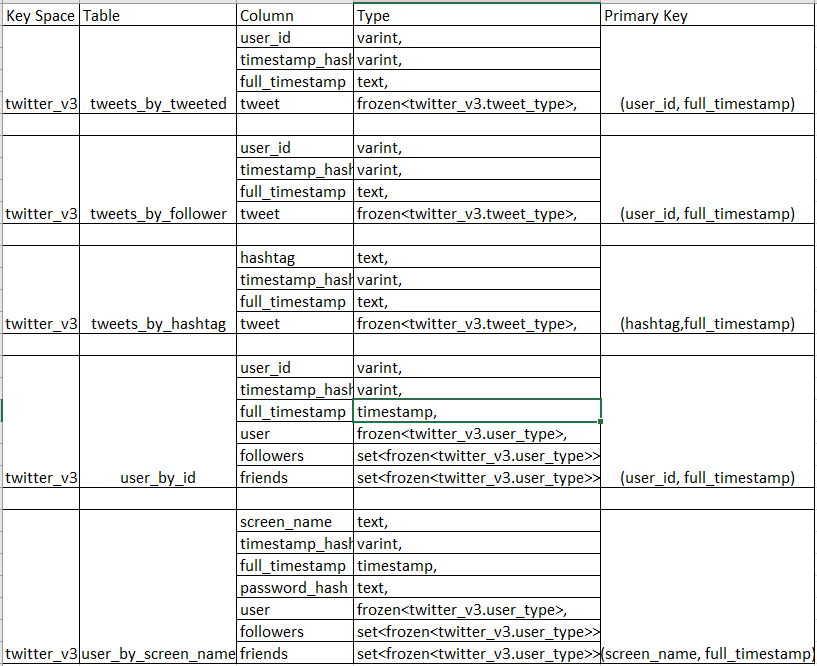
\includegraphics[scale=0.5, draft]{pics/schema.png}
	\caption{Cassandra Schema}
	\label{fig:schema}
\end{figure}
Da man bei Cassandra nur über den Primary Key (PK) auf Zeilen zugreifen und Bereichsabfragen über CQL machen kann, gilt es hier den PK so zu wählen, dass alle unsere Funktionen abgedeckt sind. Deshalb haben wir bei neben der User-Id für user\_by\_id und dem Screen-Name der Users für user\_by\_screen\_name auch den Timestamp mit aufgenommen. Da Cassandra leider keine vollständige Konsistenz bietet, müssen wir uns selber darum kümmern. Durch den Timestamp können wir verschiedene Versionen eines Objektes auseinander halten und die neuste bestimmen. Somit können wir zumindest einen gewissen Grad an Konsistenz bieten. Die weiteren Attribute der beiden Tabellen lassen sich einfach erklären. Die Follower und Friends eines Users sind wichtig, um die Timeline zu erstellen. Den password\_hash in user\_by\_screen\_name brauchen wir für den Login.\\
Die anderen drei Tabellen sind dafür da, die Tweets zu speichern und alle Tweet betreffenden Anfragen zu beantworten. Auch hier haben wir wieder den Timestamp bei allen Tabellen mit in den PK aufgenommen um Teilkonsistenz zu gewährleisten. tweets\_by\_tweeted speichert alle Tweets nach der User-Id des Users ab, der den Tweet abgesetzt hat. tweets\_by\_follower hingegen speichert einmal alle Tweets nach User-Id eines jeden Followers ab. Das Konzept hier ist es, durch die mehrfache Speicherung eines Tweets die Zeit bei der Abfrage nach allen Tweets, die ein User auf seiner Timeline sehen kann, zu verkürzen. Da man einmal abgesetzte Tweets auch nicht mehr ändern kann haben wir auch kein Problem damit jedes Objekt für Änderungen wieder heraussuchen zu müssen. tweets\_by\_hashtag speichert dann die Tweets danach ab, welche Hashtags in ihnen verwendet werden. Somit können auch Abfragen über Tweets eines Hashtags effizient beantwortet werden.

\section{Cassandrareader}
Die zentrale Applikation in der alle Funktionen und Schnittstellen umgesetzt werden ist der cassandrareader. Es ist eine modular aufgebaute in Java geschriebene Anwendung. Als Framework zur Unterstützung von verschiedenen Funktionen haben wir uns für SpringBoot entschieden. SpringBoot hat den Vorteil, dass es eine native API für Kafka besitzt, die es uns sehr leicht ermöglicht Publisher und Subscriber für Kafka-Topics zu schreiben. So ist die Verbindung mit Kafka sehr einfach konfigurierbar und kann innerhalb von kurzer Zeit verwendet werden. Für die Verbindung von Java zu Cassandra haben wir der DataStax Treiber genutzt \cite{DataStax}. Er biete eine generische Schnittstelle über die man mit Cassandra über CQL kommunizieren kann. Da er gut dokumentiert ist und es sehr viele Beispiele für verschiedene Anwendungen im Internet gibt, verlief die Einarbeitung in die Nutzung des DataStax Treibers sehr schnell.
\begin{figure}[htbp]
	\centering
	\includegraphics[scale=0.5, draft]{pics/cassandrareader_stack.png}
	\caption{Technologie Stack des cassandrareaders}
	\label{fig:techStackCass}
\end{figure}
Alle hier und im folgenden genutzten Bibliotheken werden über Maven eingebunden und der Applikation so zur Verfügung gestellt. Somit ist sichergestellt, dass immer die richtige Version geladen wird und keine Kompatibilitätsprobleme entstehen.

\subsection{Architektur}
Der Aufbau des Cassandrareaders ist sehr einfach gehalten wie man in Abbildung \ref{fig:archCass} sehen. Die Verbindung zu Cassandra wird vom Singleton CassandraConnector gemanaged. Diese Klasse stellt die Verbindung zu Cassandra her und bietet verschiedene Methoden an, Abfragen an Cassandra über CQL abzusetzen. Die eigentlich Funktion und Implementierung der Use Cases geschieht aber in den Kafka Subscribern. Dazu gibt es eine abstrakte Klasse AbstractKafkaSubscriber, die sozusagen die Infrastruktur bereitstellt. Diese besteht aus dem CassandraConnector, eine Gson-Instanz und mehreren Methoden, die die Optimierungen der Methoden aus dem Cassandra Connector darstellen, wie z.B. Batch-Queries und asynchrone Queries. Die Gson-Instanz kommt von der Google Gson Bibliothek, die für die JSON Konvertierung von Java Klasse zuständig ist. Sie wird in den abgeleiteten Klassen so benutzt, dass Kafka-Anfragen direkt in POJO Objekte gemappt werden, aus denen man dann alle relevanten Informationen bekommt. In den abgeleiteten Klassen wird dann auch die eigentliche Funktion eines Use Cases implementiert.
\begin{figure}[htbp]
	\centering
	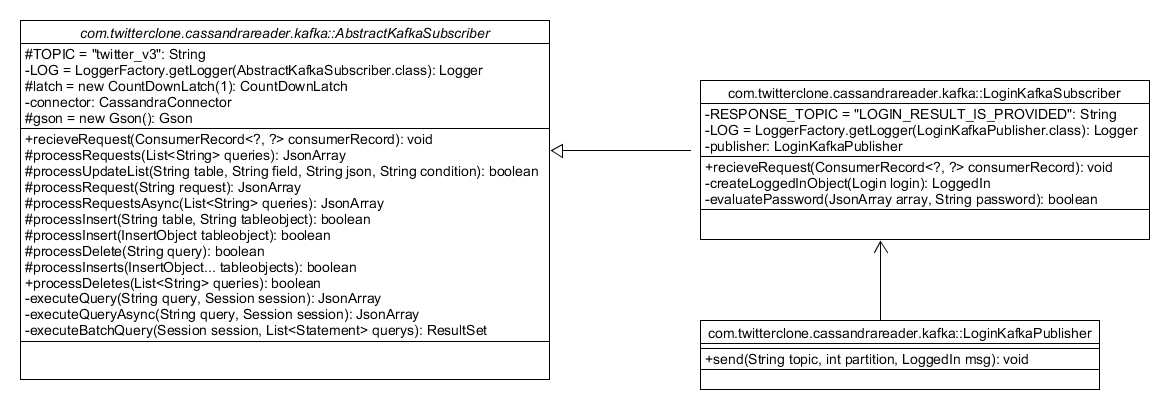
\includegraphics[scale=0.25, draft]{pics/cassandrareader_architecture.png}
	\caption{Technologie Stack des cassandrareaders}
	\label{fig:archCass}
\end{figure}
Alle möglichen Anfragen und Antworten über Kafka sind als Java Klassen modelliert und können über Getter-Methoden abgefragt werden. Jeder der abgeleiteten Subscriber besitzt einen Publisher, über den die Antwort, durch Gson konvertiert, wieder versendet werden kann. Die Konfigurationsparameter sind in der application.properties abgelegt und werden in den einzelnen Klassen angesprochen.


\section{Use Cases}
\label{sec:usecase}
Bei der Identifizierung der Use Cases die für Cassandra relevant sind haben wir uns für die Funktionen entschieden, die für einen Twitter-Client nach MVP-Prinzip (Minimal Viable Product) notwendig sind. Dabei haben wir vor allem die dazu gehören folgende Funktionen:
\begin{itemize}
	\item Registrierung von User
	\item Anmelden von Usern
	\item Abrufen der Timeline:
		\begin{itemize}
			\item Abfragen von Tweets
			\item Abfragen von Usern
		\end{itemize}
	\item Absenden/Speichern von Tweets
\end{itemize}
Diese Schnittstellen machen es möglich die Grundfunktionen, also das Erstellen eines Users, das Anmelden, das Senden von Tweets und das Lesen von Tweets über die Timeline von außen über vordefinierte Kafka Nachrichten anzusprechen.
Als weitere Schnittstellen für erweiterte Funktionen haben wir eine API für Volltextsuche über Elasticsearch gebaut, die die normale Volltextsuche aber auch Autocompletion unterstützt.\\ \TODO{vielleicht deletion hinzufügen}




\subsection{Registrierung von Usern}

\subsection{Anmelden von Usern}

\subsection{Abfragen von Tweets}

\subsection{Abfragen von Usern}

\subsection{Abrufen der Timeline}

\subsection{Absenden/Speichern von Tweets}



\chapter{Conclusion}
Write here you conclusions

\section{Future work}




\blankpage

% usare questo invece di usare \appendix perchè l'altro dà un ref sbagliato sul primo link dell'indice
\begin{appendices}
	\chapter{Glossary}
\label{appendixA}
Just comment \verb|\chapter{Glossary}
\label{appendixA}
Just comment \verb|\chapter{Glossary}
\label{appendixA}
Just comment \verb|\input{AppendixA-Glossary.tex}| in Masterthesis.tex if you don't need it!

\begin{longtable}{p{2.5cm}p{9.5cm}}

\huge{\textbf{Symbols}}& \\
\hline
\\
\$ & US. dollars. \\
\\
\\
\huge{\textbf{A}}& \\
\hline
\\
A& Meaning of A.\\
\\
\\
\huge{\textbf{B}}& \\
\hline
\\

\\
\\
\huge{\textbf{C}}& \\
\hline
\\

\\
\\
\huge{\textbf{D}}& \\
\hline
\\

\\
\\
\huge{\textbf{E}}& \\
\hline
\\

\\
\\
\huge{\textbf{F}}& \\
\hline
\\

\\
\\
\huge{\textbf{G}}& \\
\hline
\\
\\
\\
\huge{\textbf{H}}& \\
\hline
\\

\\
\\
\huge{\textbf{I}}& \\
\hline
\\

\\
\\
\huge{\textbf{J}}& \\
\hline
\\

\\
\\
%\huge{\textbf{K}}& \\
%\hline
%\\
%\\
%\\
%\huge{\textbf{L}}& \\
%\hline
%\\
%\\
%\\
\huge{\textbf{M}}& \\
\hline
\\

\\
\\
\huge{\textbf{N}}& \\
\hline
\\

\\
\\
%\huge{\textbf{O}}& \\
%\hline
%\\
%\\
%\\
\huge{\textbf{P}}& \\
\hline
\\

\\
\\
\huge{\textbf{Q}}& \\
\hline
\\

\\
\\
\huge{\textbf{R}}& \\
\hline
\\

\\
\\
\huge{\textbf{S}}& \\
\hline
\\

\\
\\
\huge{\textbf{T}}& \\
\hline
\\

\\
\\
\huge{\textbf{U}}& \\
\hline
\\

\\
\\
\huge{\textbf{V}}& \\
\hline
\\

\\
\\
\huge{\textbf{W}}& \\
\hline
\\

\\
\\
\huge{\textbf{X}}& \\
\hline
\\

\\
\\
%\huge{\textbf{Y}}& \\
%\hline
%\\
%\\
%\\
%\huge{\textbf{Z}}& \\
%\hline
%\\
%\\
%\\
\end{longtable}



| in Masterthesis.tex if you don't need it!

\begin{longtable}{p{2.5cm}p{9.5cm}}

\huge{\textbf{Symbols}}& \\
\hline
\\
\$ & US. dollars. \\
\\
\\
\huge{\textbf{A}}& \\
\hline
\\
A& Meaning of A.\\
\\
\\
\huge{\textbf{B}}& \\
\hline
\\

\\
\\
\huge{\textbf{C}}& \\
\hline
\\

\\
\\
\huge{\textbf{D}}& \\
\hline
\\

\\
\\
\huge{\textbf{E}}& \\
\hline
\\

\\
\\
\huge{\textbf{F}}& \\
\hline
\\

\\
\\
\huge{\textbf{G}}& \\
\hline
\\
\\
\\
\huge{\textbf{H}}& \\
\hline
\\

\\
\\
\huge{\textbf{I}}& \\
\hline
\\

\\
\\
\huge{\textbf{J}}& \\
\hline
\\

\\
\\
%\huge{\textbf{K}}& \\
%\hline
%\\
%\\
%\\
%\huge{\textbf{L}}& \\
%\hline
%\\
%\\
%\\
\huge{\textbf{M}}& \\
\hline
\\

\\
\\
\huge{\textbf{N}}& \\
\hline
\\

\\
\\
%\huge{\textbf{O}}& \\
%\hline
%\\
%\\
%\\
\huge{\textbf{P}}& \\
\hline
\\

\\
\\
\huge{\textbf{Q}}& \\
\hline
\\

\\
\\
\huge{\textbf{R}}& \\
\hline
\\

\\
\\
\huge{\textbf{S}}& \\
\hline
\\

\\
\\
\huge{\textbf{T}}& \\
\hline
\\

\\
\\
\huge{\textbf{U}}& \\
\hline
\\

\\
\\
\huge{\textbf{V}}& \\
\hline
\\

\\
\\
\huge{\textbf{W}}& \\
\hline
\\

\\
\\
\huge{\textbf{X}}& \\
\hline
\\

\\
\\
%\huge{\textbf{Y}}& \\
%\hline
%\\
%\\
%\\
%\huge{\textbf{Z}}& \\
%\hline
%\\
%\\
%\\
\end{longtable}



| in Masterthesis.tex if you don't need it!

\begin{longtable}{p{2.5cm}p{9.5cm}}

\huge{\textbf{Symbols}}& \\
\hline
\\
\$ & US. dollars. \\
\\
\\
\huge{\textbf{A}}& \\
\hline
\\
A& Meaning of A.\\
\\
\\
\huge{\textbf{B}}& \\
\hline
\\

\\
\\
\huge{\textbf{C}}& \\
\hline
\\

\\
\\
\huge{\textbf{D}}& \\
\hline
\\

\\
\\
\huge{\textbf{E}}& \\
\hline
\\

\\
\\
\huge{\textbf{F}}& \\
\hline
\\

\\
\\
\huge{\textbf{G}}& \\
\hline
\\
\\
\\
\huge{\textbf{H}}& \\
\hline
\\

\\
\\
\huge{\textbf{I}}& \\
\hline
\\

\\
\\
\huge{\textbf{J}}& \\
\hline
\\

\\
\\
%\huge{\textbf{K}}& \\
%\hline
%\\
%\\
%\\
%\huge{\textbf{L}}& \\
%\hline
%\\
%\\
%\\
\huge{\textbf{M}}& \\
\hline
\\

\\
\\
\huge{\textbf{N}}& \\
\hline
\\

\\
\\
%\huge{\textbf{O}}& \\
%\hline
%\\
%\\
%\\
\huge{\textbf{P}}& \\
\hline
\\

\\
\\
\huge{\textbf{Q}}& \\
\hline
\\

\\
\\
\huge{\textbf{R}}& \\
\hline
\\

\\
\\
\huge{\textbf{S}}& \\
\hline
\\

\\
\\
\huge{\textbf{T}}& \\
\hline
\\

\\
\\
\huge{\textbf{U}}& \\
\hline
\\

\\
\\
\huge{\textbf{V}}& \\
\hline
\\

\\
\\
\huge{\textbf{W}}& \\
\hline
\\

\\
\\
\huge{\textbf{X}}& \\
\hline
\\

\\
\\
%\huge{\textbf{Y}}& \\
%\hline
%\\
%\\
%\\
%\huge{\textbf{Z}}& \\
%\hline
%\\
%\\
%\\
\end{longtable}



\blankpage
	\chapter{Cassandra}
\label{appendix:Cassandra}
Cassandra ist eine NoSql Datenbank, die nach dem Wide-Column Model konzipiert ist. Cassandra vereint verschieden Eigenschaften von Googles BigTable \cite{bigtable} und Amazons Dynamo \cite{dynamo}. Sie wurde 2010 von Facebook entwickelt, um das Inbox Search Problem zu lösen \cite{cassandra}. Es ist eine verteilte Datenbank, die sich unter dem CAP-Theorem als AP charakterisieren lässt, wobei man das Level an Konsistenz manuell einstellen kann.

\section{Daten Model}
\label{sec:DM}
Das Daten Modell von Cassandra entspricht dem von BigTable, also dem Wide-Column Modell. Dies beruht im Wesentlichen, wie alle Arten an NoSql Datenbank Modellen auf Key-Value-Stores. Dabei wird für einen Primary Key jeweils eine Reihe mit Column-Families definiert. Die Column-Families bestehen wiederum aus einem Key, der sie beschreibt, und einem Value der dann den Wert angibt. Der Wert kann allerdings wieder eine Menge an Column-Families sein, wodurch es möglich ist Column-Families beliebig zu verschachteln. Es wird bei der Initialisierung angegeben welchen Typ der Wert hat, Verschachtlung wird über benutzerdefinierte Typen erzeugt.
\begin{figure}[htbp!]
	\centering
	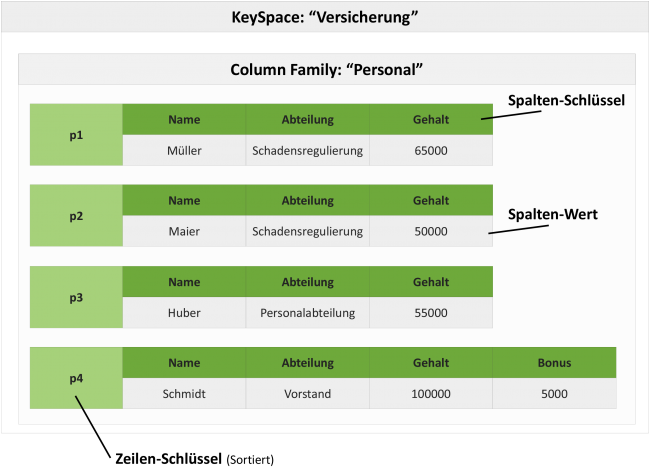
\includegraphics[scale=0.45]{pics/colfam.png}
	\figuresource{\url{http://wi-wiki.de/doku.php?id=bigdata:spaltendb}}
	\caption{Beispiel Daten Modell}
	\label{fig:bspDM}

\end{figure} Column-Families, die wiederum Column-Families beinhalten, bezeichnet man als Super-Column-Families. Bei Cassandra werden bei der Initialisierung einer Tabelle, die auch nichts anderes ist als eine Super-Column-Family, alle möglichen Column-Families angegeben. Sie definiert darüber hinaus den Primary Key über den auf die Werte der Column-Families zugegriffen werden können. Im Unterschied zu herkömmlichen SQL Tabellen ist es aber möglich Werte für diese zu unterschlagen, wie in Abbildung \ref{fig:bspDM} für p1 - p3 dargestellt.\\ 
Ein KeySpace stellt die oberste Schicht des Datenmodells dar. Für den KeySpace werden bei der Initialisierung eine Replikationsstrategie und eine Anzahl Replikas angegeben, die zu erstellen sind. Diese gelten dann für alle Tabellen, die unter dem KeySpace erstellt werden.

\section{System}
Implementiert ist Cassandra in Java. Darauf aufbauend sind auch die Basis Java Typen verfügbar. Die Daten werden von Cassandra redundant auf verschiedene Instanzen verteilt. Systemnachrichten werden dabei über UDP verschickt, Anwendungsnachrichten, also Nachrichten, die mit den Daten zu tun haben, per TCP um den Verlust von Nachrichten zu vermeiden. Bei den Systemnachrichten ist dies zu verkraften.

\subsection{Partitionierung}
Die Partitionierung orientiert sich an der von Dynamo \cite{dynamo}. Cassandra benutzt genauso wie Dynamo Consistent-Hashing, um Daten auf die verschiedenen Instanzen zu verteilen. Dabei erhalten die verschiedenen Instanzen einen Wert, der sie uniform über einen vordefinierten Wertebereich verteilt, wie in Abbildung \ref{fig:uniformHashing} abgebildet. Consistent-Hashing macht aus dem Wertebereich einen Ring, über den dann die Daten auf die Instanzen wie folgt verteilt werden. Aus einem Datum wird über die Hashfunktion ein Hash-wert berechnet. Das Datum wird dann auf der Instanz abgespeichert, deren Wert auf dem Ring aufsteigend als nächstes kommt. Dieses Verfahren kann zu einer ungleichen Verteilung der Daten auf die Instanzen führen, sodass dadurch die Performance des Systems ineffizient wird. Cassandra löst diese Problem anders als Dynamo dadurch, dass die Werte der Instanzen an die Verteilung der Daten angepasst werden, wie in Abbildung \ref{fig:adaptedHashing} dargestellt. So sind zwar einige Instanzen für einen größeren Wertebereich zuständig, andererseits kommen in diesem größeren Wertebereich weniger Daten vor, sodass die Daten uniform auf die Instanzen verteilt werden. Wird der Datensatz zu groß, skaliert Cassandra, indem eine Instanz im Consistent-Hashing Ring zwischen den Knoten mit den meisten Daten eingefügt wird. Danach werden die Bereiche wieder so angepasst, dass alle Instanzen ungefähr gleich belastet sind.
\begin{figure}[htbp!]
	\centering
	\begin{subfigure}[c]{0.49\textwidth}
		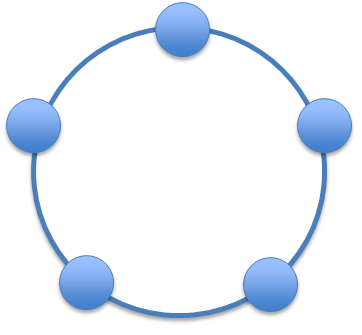
\includegraphics[scale=0.5]{pics/uniformHashing.png}
		\subcaption{Consistent-Hashing uniform distributed instances}
		\label{fig:uniformHashing}
	\end{subfigure}
	\begin{subfigure}[c]{0.49\textwidth}
		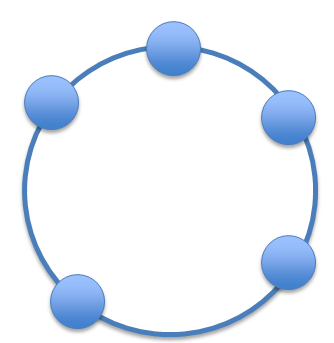
\includegraphics[scale=0.5]{pics/adaptedHashing.png}
		\subcaption{Consistent-Hashing adapted distribution of instances}
		\label{fig:adaptedHashing}
	\end{subfigure}
	\caption{Consistent-Hashing Ring}
\end{figure}

\subsection{Replikation}
Die Art der Replikation in Cassandra ist vom Benutzer konfigurierbar. Die Anzahl der Replikas und die Replikationsstrategie wird durch den KeySpace festgelegt. Dabei kann man zwischen SimpleStrategy und NetworkTopologyStrategy auswählen. Die SimpleStrategy repliziert ohne auf die Netzwerkstruktur einzugehen. Somit beugt sie weniger stark potentiellem Datenverlust vor und sollte daher nur für Test-Zwecke benutzt werden. Sei N die Anzahl Replikas, werden die Daten immer auf die N-1 Nachfolgeknoten repliziert. Bei der NetworkTopologyStrategy wird die Hierarchie von Datacentern und drin enthalten Racks bei der Verteilung betrachtet wird. Somit wird diese Strategie auch für das Deployment empfohlen. Innerhalb dieser Strategie kann man sich wiederum zwischen Rack Aware und Datacenter Aware entscheiden. Dabei werden die Replikas entweder auf verschiedene Racks oder Datacenter verteilt, um die höchst mögliche Datensicherheit zu gewährleisten. Diese Strategien beziehen sich auf den Koordinator, also die Hauptinstanz einer Partition von Daten, da dieser für die Replikation zuständig ist.
Bei der Bestimmung eines Koordinators wird Zookeeper verwendet. Dadurch sind alle Netzwerkänderungen und -konfigurationen persistent gespeichert, da Zookeeper die Konfigurationen jedes Knotens automatisch persistent speichert. Zur Kommunikation werden bei Zookeeper Gossip Algorithmen verwendet.

\subsection{Persistenz}
Persistenz erreicht Cassandra über ein ähnliches System wie BigTable \cite{bigtable}. Zunächst gibt es die MemTable, die im Hauptspeicher gehalten wird und als Cache fungiert. Sie besitzt eine Konfiguration einer Schranke, ab der die MemTable auf die Platte persistiert wird. Auf der Platte gibt es die SSTable, Bloom Filter, index file, compression file und statistics file. Die Daten werden in eine SSTable geschrieben, also eine eigene Datei geschrieben, wenn sie noch nicht vorhanden sind. Wenn dies nicht der Fall ist, wird der betreffende Teil einer SSTable in die MemTable geladen, alle Operationen ausgeführt und die Daten wieder zurück auf die Platte geschrieben. Der Bloom Filter verhindert unnötige Lookups in nicht relevante SSTables. Der Index beschleunigt den Lookup innerhalb einer SSTable. Damit man nicht viele kleine SSTable-Dateien hat werden zwei SSTable, durch einen merge-Prozess immer dann zusammengefasst, wenn eine mindestens halb so groß ist wie die andere. Vorhandene SSTable Files können zusätzlich noch komprimiert werden.

\section{CQL}
Mit CQL (Cassandra Query Language) gibt es eine auf Cassandra zugeschnittene SQL-ähnliche Abfragesprache, die es den Anwendern konventioneller Datenbanken deutlich leichter macht mit Cassandra zu arbeiten. Dabei ist es wichtig zu wissen, dass CQL bei weitem nicht so ausdrucksstark ist wie SQL. Das liegt daran, dass CQL im wesentlich eine abstrakte API für das Cassandra Datenmodell darstellt. In CQL sind normale Datenbank Typen wie int, text, etc. möglich, allerdings kann man auch von Collections wie List, Set und Map Gebrauch machen, da es dafür direkte Java Typen gibt. Des Weiteren ist es möglich eigene Typen zu definieren, wie schon in Abschnitt \ref{sec:DM} beschrieben.\\
\begin{figure}[htbp!]
	\centering
	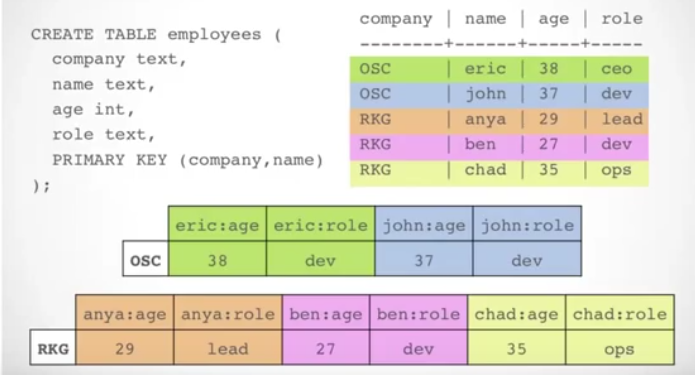
\includegraphics[scale=0.7]{pics/cql_mapping.png}
	\figuresource{\url{https://www.youtube.com/watch?v=UP74jC1kM3w}}
	\caption{CQL Mapping}
	\label{fig:mapping}
\end{figure}
Tabellen und Spalten werden wie ebenso in Abschnitt \ref{sec:DM} beschrieben durch Column-Families dargestellt. und wie in SQL erzeugt. Dabei wird ein Primary Key benötigt, der dann als Row Key fungiert. Es kann nur über diesen Row Key auf die Zeilen zugegriffen werden. Deshalb kann man in der WHERE-Klausel in CQL auch nur Elemente des Primary Key angeben. Auf diesen Elementen wird durch die Indizierung schon beim Speichern in Cassandra eine Sortierung berechnet was die Anfragen deutlich perfomanter macht. Für alle anderen Spalten der Zeile wäre dies also nicht performant und wird von CQL nicht gestattet. Die Spalten und Zeilen werden wie folgt auf das Cassandra Datenmodell abgebildet.\\
Der erste Teil des Primary Keys bildet, wie man sehen kann, den Row Key, die restlichen Teile werden mit ihren Werten in die Beschreibung der Column-Families integriert, so wie im unteren Teil in Abbildung \ref{fig:mapping} beschrieben. Somit werden alle Zeilen mit dem gleichen ersten Teil des Primary Keys in der gleichen Zeile abgespeichert. Über dieses Mapping ist es möglich eine tabellenartige Abstraktion zu erzeugen, die sich durch CQL ausdrückt und Anwendern ein aus SQL bekanntes Interface bietet.

	\chapter{Big Table}
\label{bigTable}
Some text.

\section{Einführung}
Täglich kommen mehrere Petabytes an Daten von über 60 Google Anwendungen zusammen. Dafür verantwortlich sind mehr als 1000 Computer die untereinander vernetzt sind. Um diese Daten verwalten zu können wurde Bigtable ins Leben gerufen. Das Ziel der Datenbank war es in vielen Bereichen anwenden zu können. Dazu sollte es Skalierbar sein sowie eine hohe Performance und Verfügbarkeit besitzen.


\section{Datenmodell}
Bigtable ist eine verteiltes, persistentes multidimensionale sortierte Map. Diese Map ist indexiert über eine row key, columen key und einem timestamp. Jeder Wert in dieser Map ist ein Array mit Bytes. Das folgende Datenmodell soll eine Speicherung von Webseiten veranschaulichen.

\begin{figure}[!htpb]
	\centering
	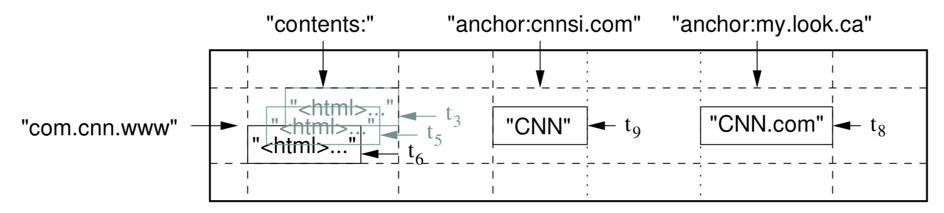
\includegraphics[]{pics/bigtable_schema.png}
	\caption {Tabellen Beispiel}	
\end{figure}

Das Datenmodell besteht aus zwei Familien dem Inhalt und den Ankerpunkten. Die erste Familie beinhaltet den Inhalt der Webseite, mit drei unterschiedlichen Zeitstempeln (t3,t5,t6). Drei unterschiedliche Zeitstempeln bedeutet, dass die Website www.cnn.com in drei unterschiedlichen Versionen abgespeichert wurde. Die Anker Familie beinhaltet jeweils nur eine Version. Den Anker mit „CNN.com“ mit dem Zeitstempel t8 und dem Anker „CNN“ mit dem Zeitstempel t9. 
 
\paragraph{Rows}
Bigtable speichert Daten in lexikopgrahischer reihenfolge und sortiert diese nach Zeilen. Eine row range beinhaltet alle gleichnamigen URL’s, so dass alle mit der gleichen Domain zusammen abgespeichert werden. Das vereinfacht die Analyse und das Hosting der gleichnamigen Domains und macht dies zudem effizienter.

\paragraph{Column families}
Verschieden column keys werden in eine gemeinsame Gruppe gespeichert. Das nennt man column families. Alle Daten, welche in der gleichen Gruppe gespeichert werden sind vom gleichen typ. Bevor Daten in einer Gruppe gespeichert werden können, muss diese column family als erstes erstellt werden.

\paragraph{Timestamp}
Jede Zelle in Bigtable kann mehrere Versionen der gleichen Daten beinhalten. Dieser Versionen werden indexiert durch den Zeitstempel (timestamp). Der Zeitstempel ist bis auf die Micro Sekunde genau. Durch die „two per-column-family“ kann der Benutzer festlegen, wie viele Versionen der gleichen Daten gespeichert werden sollen. Alle weiteren Versionen werden automatisch gelöscht.

\paragraph{API}
Die API von Bigtable ermöglicht das erstellen und löschen von Tabellen und Spaltennamen, sowie das ändern von Tabellen, Cluster und Metadaten einer Spaltenfamilien. Das folgende Codebeispiel wurde in C++ geschrieben und Verändert den Inhalt der Tabelle Webtable. 

\begin{figure}[!htpb]
	\centering
	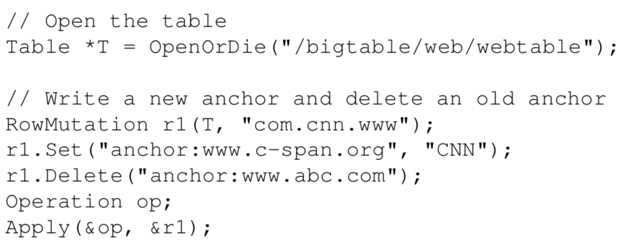
\includegraphics[]{pics/bigtable_api.png}
	\caption {Zugriffs Beispiel mit der BigTable API}	
\end{figure}

Der Code verändert die Spalte „com.cnn.www“ und fügt einen neuen Anker hinzu. Im nächsten Schritt wird ein vorhandener Anker „anchor:www.abc.com“ gelöscht und festgeschrieben.


\paragraph{Building Blocks}
Bigtable ist auf mehreren anderen Teilen der Google-Infrastruktur aufgebaut. Zum Beispiel benutzt Bigtable das verteilte Google File System (GFS). Welches für die Speicherung von Logs und Daten verantwortlich ist. Ein Bigtable Cluster operiert typischerweise auf einem verteilten Pool von Computern. Auf diesem Pool laufen eine breite sparte von verschiedenen Anwendungen. Bigtable basiert auf einem Cluster Management System für Zeit-Planung-Jobs, Ressourcenmanagements auf geteilten Computer, agieren mit Computerfehlern und dem Anzeigen des Computer Status. Das SSTable Format stellt eine persistente, geordnete unveränderliche Abbildung von Schlüsseln zu Werten zur Verfügung, wobei sowohl Schlüssel als auch Werte willkürliche Bytefolgen sind. Operationen werden bereitgestellt, um den Wert zu suchen, der einem bestimmten Schlüssel zugeordnet ist.

\paragraph{Implementation}
Bigtable besteht aus drei Haupt Komponenten, einer Bibliothek, einem Master Server und vielen weiteren tablet servern. Die Bibliothek ist in jeden Client verlinkt, somit kann der Client auf alle Funktionen zugreifen. Der Master Server wird zufällig ausgewählt. Dieser teilt den tablet servern die tablets zu. Außerdem ist für die Verteilung der Lasten zuständig und ist für die garbage collection. Sobald eine Tabelle zu groß wird, wird diese von einem tablet server gesplittet. So wird sichergestellt, dass eine Tabelle nie größer als 100-200 MB ist.

\paragraph{Tablet location}
Um Daten zu speichern, verwendet Google bei Bigtable eine „three-level hirarchy“. Das erste Level ist eine Datei, welches auch das Chubby file genannt wird, dort wird der Speicherort des root tablets hinterlegt. Das root tablet beinhaltet alle Speicherorte aller tablets in einer METADATA Tabelle. Das spezielle an dieser Tabelle ist, dass egal wie groß sie wird, diese niemals geteilt wird. Somit wird sichergestellt, dass die „three-level hirarchy“ eingehalten wird. Die METADATA Tabellen speichern die Orte aller anderen tablets in einer Tabelle ab.

\paragraph{Tablet Zuweisung}
Jedes tablet ist zu einem Zeitpunkt immer nur einem tablet server zugeordnet. Der Master server verfolgt die lebenden tablet servern und die aktuell zugeordneten tablets zu den tablet servern inklusive aller unzugeordneten tablet servern.
Beim Start einer Bigtable führt der Master Server folgende Schritte aus:

\begin{enumerate}
	\item Wählt einen einzigartigen Master Lock in Chubby
	\item Scannt die Server Verzeichnisse um die lebenden tablet server zu finden
	\item Kommuniziert mit den vorhandenen tablet server um bereits zugeordnete tablets zu identifizieren
	\item Master scannt METADATA Tabelle um die vorhandene Zugehörigkeiten zu lernen
\end{enumerate}

\paragraph{Tablet serving}
Ein persistenter Zustand eines tablets wird in GFS gespeichert. Alle Updates werden auf „well-formed“ geprüft und anschließend in einem commit-log gespeichert. Die neusten Updates werden in eine memtable gespeichert, ältere updates werden in die SSTable geschrieben. Wenn Daten aus dem tablet server abgefragt werden muss ein merge zwischen den neuen Daten in der memtable sowie den älteren Daten in der SSTable erstellt werden.

\paragraph{Compaction}
Je mehr Daten gespeichert werden, umso größer wird die memtable. Damit diese tabelle nicht zu groß wird, gibt es ein „minor compaction“. Diese Funktion friert eine memtable ein sobald diese eine bestimmte Größe erreicht hat und erstellt eine neue memtable. Die gefrorene memtable wird zu einer SSTable konvertiert. Je mehr Daten gespeichert werden, desto unordentlicher wird die Ansammlung von SSTable. Um die SSTable zu sortieren wird periodisch ein „merging compaction“ ausgeführt. Dies strukturiert die SSTable neu und es werden Ressourcen, durch die Löschung von Daten, freigegeben. Außerdem werden gelöschte Daten endgültig gelöscht, das ist wichtig für Services, welche sensible Daten beinhalten.

\section{Refinments}
Um die hohe Performance, Verfügbarkeit und Zuverlässigkeit beizubehalten, werden einige Verbesserungen (refinments) benötigt.

\paragraph{Lokale Gruppen}
Gruppierung erspart Zugriffszeit. Zum Beispiel bei dem Datenmodell Webseite. Die „page metadate“ und „content“ der Webseite werden in einer anderen gruppe gespeichert. So muss eine Anwendung, welche nur die Metadaten möchte, nicht durch den kompletten Inhalte einer Seite iterieren.
Zudem gibt es Tuningparameter, welche bestimmten ob Daten in den Arbeitsspeicher geladen werden um die Zugriffszeit zu minimieren.

\paragraph{Kompression}
Ein Benutzer kann selbst bestimmen ob SSTable komprimiert wird und falls ja, in welchem Ausmaß. Jeder SSTable Block kann einzeln ausgewählt werden. Für die Komprimierung kommen die  verfahren Bentley und McLlroy’s zum Einsatz. Diese können mit 100-200Mb/s Kodiert und mit 400-1000 MB/s Enkodiert werden.

\paragraph{Caching für Lesezugriffe}
Für das Caching von Lesezugriffe gibt es zwei verfahren. Der Scan Cache (high-level), speichert key-value Paare und liefert eine SSTable zurück. Das Block Cache (lover-level) verfahren speichert SSTable Blocks, die von der GFS gelesen werden.

\paragraph{Bloom Filter}
Benutzer legt selbst fest ob ein Filter zum Einsatz kommt. Der Vorteil eines Filters liegt darin, dass wenn Daten gesucht werden, nicht jede SSTable nach den bestimmten Daten durchsucht werden muss. Ein Bloom Filter erlaubt es, nach einer bestimmten Art von row/column paaren zu fragen, ob diese in einer SSTable gespeichert sind.

\paragraph{Beschleunigte tablet Wiederherstellung}
Wenn der Master ein tablet von einem Server zu einem anderen Server verschiebt, führt der Ursprungs Server erst ein „minor compaction“ aus um die Ladezeit für den neuen tablet server zu verkürzen.

\paragraph{Unveränderlichkeit ausnutzen}
Es können nur Daten verändert, welche in der memtable stehen. Daten in der SSTable können nicht verändert werden. Das macht man sich zu nutzen indem man keine Synchronisation braucht, wenn auf die Daten zugegriffen wird. Memtable sind die einzigen Daten auf die man schreiben kann und gleichzeitig lesen. Damit es zu keinen komflikten kommt, setzt Bigtable hier auf „Copy-on-write“. 

\section{Performance Auswertung}
\begin{figure}[!htpb]
	\centering
	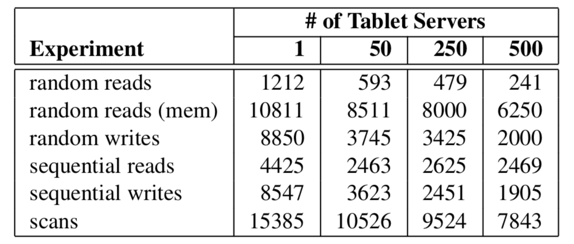
\includegraphics[]{pics/bigtable_performance.png}
	\caption {Percormance Übersicht}	
\end{figure}
Die Performance wird hauptsächlich durch die verwendete CPU (2ghz) begrenzt. Zudem kann man erkennen, dass bei einem tablet server der Durchsatz bei ca. 75MB/s liegt (1000 bytes * 64 KB Block size = 75 MB/s). Damit der Durchsatz bei einem Single tablet server erhöht wird, wird die die SSTable größe in der regel von 64KB auf 8kb gesenkt. 
Zudem wird erkannt, dass der Durchsatz nicht Linear ansteigt. Bei einer Erhöhung der tablet server von eins auf 500 liegt die Erhöhung des Durchsatzes bei gerade mal dem 300 fachen (10811 / (500 * 6250) = 350). Diese Begrenzung liegt wie bei einem tablet server an der CPU der tablet servern.

	\chapter{Dynamo}
\label{appendiceC}


\section{Problemstellung und Einordnung}
Amazon wickelt Bestellungen von Kunden rund um die Welt ab. Hierfür benötigt Amazon ein hochverfügbares System, das sicherstellt, dass jederzeit Bestellungen entgegen genommen werden können. Es werden also viele Rechenzentren benötigt, um diese Last zu tragen. Bei der Auswahl von Rechnern für diese Rechenzentren setzt Amazon allerdings nicht auf hochverfügbare Spezialhardware, sondern setzt handelsübliche Rechner ein. Um dennoch eine möglichst hohe Verfügbarkeit garantieren zu können, hat Amazon die verteilte Datenbank Dynamo entwickelt, die in \cite{dynamo} beschrieben wurde und in diesem Kapitel vorgestellt werden soll. \\ 
\\
Dynamo ist dafür konzipiert, bei Verfügbarkeit einer minimalen Anzahl an Knoten, Schreibvorgänge annehmen zu können. Dynamo ist also partitionierungstolerant und hoch verfügbar, kann Datenkonsistenz aber nur unter bestimmten Bedingungen garantieren. 
\section{Datenmodell}
Dynamo ist ein Key-Value-Store. Werte werden also unter einem Schlüssel abgelegt und können nur über diesen Schlüssel wieder abgefragt werden. Komplexere Anfragen sind daher nicht möglich. Der Wert, der hinterlegt wird, muss keinem festen Datenschema entsprechen - es können beliebige Binärdaten gespeichert werden.

\section{Architektur}

\subsection{Konsistentes Hashing}
Um die Daten den Knoten zuzuordnen, verwendet Dynamo konsistentes Hashing. Hierbei wird für jeden Schlüssel ein MD5 128 Bit Hash-Wert gebildet. Den Knoten wird ebenfalls ein Wert zwischen $0$ und $2^{128}$ zugeordnet. Ein Schlüssel-Wert-Paar wird auf dem Knoten gespeichert, dem der nächst höhere Wert ausgehend vom Hash-Wert des Schlüssels zugeordnet wurde. Gibt es keinen Knoten, der einen höheren Wert hat, wird das Schlüssel-Wert-Paar auf dem Knoten mit dem kleinsten Wert gespeichert.\\
Visuell lässt sich dieses Verfahren wie in Abbildung \ref{fig:bspKonHash} mithilfe eines Kreises darstellen. Jeder Position auf dem Kreis wird im Uhrzeigersinn beginnend am obersten Punkt des Kreises ein Wert von $0$ bis $2^{128}$ zugeordnet. Knoten wie Schlüssel können dann anhand ihres Hash-Wertes auf dem Kreis platziert werden. Ein Schlüssel-Wert-Paar wird auf dem Knoten gespeichert, der auf dem Kreis an der nächsten Stelle im Uhrzeigersinn liegt.
\begin{figure}
	\caption{Beispiel für konsistentes Hashing. Die Daten sollen auf vier Knoten verteilt werden, wobei die Knoten gleichmäßig auf dem Kreis platziert sind.}
	\label{fig:bspKonHash}
	\centering
	\begin{tikzpicture}
		\draw (0,0) circle (2cm);
		\node[fill=black,circle,scale=0.5] (zero) at (0,2) {};
		\node[above] at (zero) {$2^{128}$ $0$};
		\node[fill=black,circle,scale=0.5] (A) at (1.41,1.41) {};
		\node[below left] at (A) {hash(A)};
		\node[fill=black,circle,scale=0.5] (K2) at (2,0) {};
		\node[fill=black,circle,scale=0.5] (B) at (1.79,-0.89) {};
		\node[left] at (B) {hash(B)};
		\node[fill=black,circle,scale=0.5] (C) at (1.41,-1.41) {};
		\node[left] at (C) {hash(C)};
		\node[fill=black,circle,scale=0.5] (K3) at (0,-2) {};
		\node[fill=black,circle,scale=0.5] (D) at (-1.79,-0.89) {};
		\node[right] at (D) {hash(D)};
		\node[fill=black,circle,scale=0.5] (K4) at (-2,0) {};
		\node[fill=black,circle,scale=0.5] (E) at (-1.79,0.89) {};
		\node[right] at (E) {hash(E)};
		\draw (3,2) rectangle (6,0.5);
		\draw (3,-2) rectangle (6,-0.5);
		\draw (-3,2) rectangle (-6,0.5);
		\draw (-3,-2) rectangle (-6,-0.5);
		\draw (zero) -- (3,2);
		\draw (K2) -- (3,-0.5);
		\draw (K3) -- (-3,-2);
		\draw (K4) -- (-3,0.5);
		\node at (4.5,1.5) {Knoten 1};
		\node at (4.5,1) {\scriptsize{Eintrag E}};
		\node at (4.5,-1) {Knoten 2};
		\node at (4.5,-1.5) {\scriptsize{Eintrag A}};
		\node at (-4.5,-1) {Knoten 3};
		\node at (-4.5,-1.5) {\scriptsize{Einträge B, C}};
		\node at (-4.5,1.5) {Knoten 4};
		\node at (-4.5,1) {\scriptsize{Eintrag D}};
	\end{tikzpicture}
\end{figure}
\subsection{Replikation}
Replikation lässt sich nun leicht realisieren, indem die Einträge nicht nur auf dem nächsten, sondern bei einem Replikationsfaktor von $n$ auf den nächsten $n$ Knoten gespeichert werden. Fällt dann ein Knoten aus, lassen sich die Einträge weiterhin auf dem jeweils nächsten Knoten auf dem Kreis auffinden. Bei einem Ausfall muss dafür gesorgt werden, dass die Bedingung, dass alle Daten auf den nächsten $n$ Knoten gespeichert sind, wieder hergestellt wird.
\subsection{Partitionierung und Verteilung}
Bei der Partitionierung aus Abbildung \ref{fig:bspKonHash} ist beim Ausfall eines Knotens das Problem, dass die nächsten $n$ Knoten (bei Replikationsfaktor $n$) die volle Last das Ausfalls tragen müssen, da die Daten, die der ausgefallene Knoten gespeichert hat, auf die nächsten $n$ Knoten repliziert werden müssen. Ist $n$ im Vergleich zur Anzahl der insgesamt verfügbaren Knoten eher klein, wäre es wünschenswert eine bessere Verteilung der Last zu erzielen. Daher platziert Dynamo die Knoten nicht direkt auf dem Kreis, sondern plaziert stattdessen virtuelle Knoten. Dabei stehen mehrere virtuelle Knoten für einen realen Knoten. Nun können die virtuellen Knoten so auf dem Kreis verteilt werden, dass auf die virtuellen Knoten eines realen Knotens die virtuellen Knoten verschiedener realer Knoten folgen. Bei dem Ausfall eines realen Knotens wird die entstehende Last also auf viele oder sogar alle realen Knoten verteilt.\\
\\
In Abbildung \ref{fig:bspKonHash} wurden die Knoten gleichmäßig auf dem Kreis verteilt. Es ließe sich nun ein Schema finden, das für virtuelle Knoten eine Verteilung auf dem Kreis bestimmt, durch die die virtuellen Knoten ebenfalls gleichmäßig auf dem Kreis verteilt werden, und dafür sorgt, dass der Ausfall eines Knotens zunächst von allen anderen Knoten getragen wird. Das Problem ist jedoch, dass das Schema nach dem Ausfall erneut ausgeführt werden müsste, um eine gleichmäßige Verteilung wieder herzustellen. Hierbei würden jedoch meist alle virtuellen Knoten neu platziert werden und es müssten viele Daten verschoben werden. Ein ähnliches Szenario würde das Hinzufügen eines Knotens hervorrufen.\\
Da der Aufwand für das Verschieben der Daten zu hoch wäre, lässt sich ein solches optimales globales Schema nicht realisieren. Stattdessen wurden von Amazon drei Strategien zur Verteilung der Daten evaluiert. Diese werden im Folgenden vorgestellt:
\subsubsection*{Strategie 1}
Die erste Strategie verteilt die virtuellen Knoten zufällig auf dem Kreis. Hierdurch lässt sich eine gute Lastverteilung bewirken, da es unwahrscheinlich ist, dass ein Knoten im Vergleich zu den anderen Knoten einen sehr viel größeren Bereich des Kreises zugewiesen bekommt. Des Weiteren ist die Wahrscheinlichkeit gering, dass auf die meisten virtuellen Knoten eines realen Knotens fast ausschließlich virtuelle Knoten eines einzigen anderen realen Knotens folgen.\\
Außerdem hat diese Strategie den Vorteil, dass das Hinzufügen eines neuen Knotens eine verteilte Operation ist: Der Knoten kann die Positionen seiner virtuellen Knoten zufällig auswählen und die realen Knoten, die die Daten seines Bereichs halten, um die Übergabe der Daten bitten. Diese Knoten können dann ihren Speicher nach Einträgen durchsuchen, die übergeben werden sollen.\\
Es wurde jedoch festgestellt, dass eben dieses Durchsuchen des Speichers eines Knotens sehr aufwändig ist, da alle Einträge überprüft werden müssen. Strategie 2 vereinfacht diesen Suchvorgang. 
\subsubsection*{Strategie 2}
Strategie 2 wurde nur für kurze Zeit eingesetzt und kann als Zwischenschritt zu Strategie 3 betrachtet werden.\\
Strategie 2 unterteilt den Kreis in gleichgroße Partitionen. Dabei muss die Anzahl der Partitionen sehr viel größer sein als die Anzahl der potentiellen virtuellen Knoten. Ein Knoten speichert immer nur die Daten einer vollen Partition. Auch Strategie 2 verteilt die virtuellen Knoten zufällig auf dem Kreis. Auf die gleiche Weise, wie bei Strategie 1 die Einträge auf die Knoten zugeordnet wurden, werden bei dieser Strategie die Partitionen den Knoten zugeordnet. Ein Knoten legt einen neuen Eintrag dann im Speicherbereich der entsprechenden Partition ab. Wird er von einem neuen Knoten aufgefordert, einen Bereich des Kreises abzugeben, muss er nicht seinen kompletten Speicher nach Einträgen durchsuchen, sondern nur die zum Bereich gehörenden Partitionen bestimmen. Hierdurch wird nicht nur der Suchaufwand beim Hinzufügen eines Knotens verringert, sondern auch der benötigte Speicher, um festzuhalten, welcher Bereich des Kreises auf welchem Knoten liegt, verringert sich immens.
\subsubsection*{Strategie 3}
Strategie 3 geht wie Strategie 2 vor, bis auf dass die Knoten nicht mehr auf dem Kreis platziert werden, sondern die Partitionen den Knoten direkt zufällig zugeordnet werden. Kommt ein neuer Knoten hinzu, erhält er von jedem Knoten die gleiche Anzahl an zufällig ausgewählten Partitionen.
\subsection{Die put()- und die get()-Operation}
Mit der put()-Operation lassen sich Daten in Dynamo anlegen. Wird die put()-Operation an einem Knoten aufgerufen, informiert dieser Knoten zunächst den nächsten erreichbaren Knoten auf dem Kreis ausgehend vom Hash-Wert des Schlüssels des neuen Eintrags. Dieser Knoten ist für das weitere Verfahren verantwortlich. Hat er die Nachricht erhalten, speichert er den Eintrag und informiert die nächsten $N-1$ Knoten auf dem Kreis über den Eintrag. Hat er von $W-1$ Knoten eine Bestätigung erhalten, dass diese den Eintrag ebenfalls gespeichert haben, kann er den Nutzer informieren, dass der Eintrag gespeichert ist. Der Nutzer erhält die Bestätigung also, wenn der Eintrag auf $W$ Knoten abgelegt ist. Anschließend wartet der verantwortliche Knoten, ob er von den restlichen Knoten eine Antwort bekommt und informiert den nächsten Knoten auf dem Kreis ebenfalls über den Eintrag, falls einer der $N-1$ Knoten nicht reagiert. Das Ziel ist also, den Eintrag $N$ Mal zu speichern. \\
Bei der get()-Operation wird die Anfrage ebenfalls zunächst an den verantwortlichen Knoten übermittelt. Dieser leitet die Anfrage an $N-1$ Knoten weiter und beantwortet die Anfrage, wenn ihm die Ergebnisse von $N-1$ anderen Knoten und sein eigenes Ergebnis zur Verfügung stehen. Um Widersprüche in den Ergebnissen auflösen zu können, wird eine Versionierung der Daten benötigt.
\subsection{Versionierung}
Dynamo verändert gespeicherte Einträge nicht, sondern behandelt eine Änderung als neue Version der Daten. Dynamo verwendet Vektoruhren, um aufzulösen, welche Version eines Eintrages neuer ist. Der Zeitstempel des alten Eintrages wird bei einem Update vom Nutzer der Datenbank mitgegeben, sodass der Knoten, der für den neuen Eintrag verantwortlich ist, einen neuen Zeitstempel erstellen kann. Findet ein Knoten zwei Einträge vor, die widersprüchliche Vektoren haben, also keine Aussage getroffen werden kann, welcher Eintrag neuer ist, speichert er beide Einträge ab und bei der nächsten Anfrage werden beide Einträge dem Nutzer übergeben. Dieser muss dann den Konflikt auflösen. \\
\\
Es gibt einige Anwendungsfälle, in denen eine solche Konfliktlösung leicht ableitbar ist. So wird in \cite{dynamo} der Anwendungsfall des virtuellen Einkaufskorbs als Beispiel genannt. Hatte ein Nutzer die Version 1 seines Einkaufkorbes und hat anschließend zwei Artikel in den Einkaufskorb gelegt, wobei beim ersten Artikel basierend auf Version 1 eine Version 2 des Einkaufskorbes erstellt wurde und beim zweiten Artikel ebenfalls basierend auf Version 1 eine Version 3 erstellt wurde, so lässt sich der Konflikt zwischen Version 2 und Version 3 leicht durch das Vereinigen der beiden Einkaufskörbe lösen. Auf diese Weise kann kein hinzugefügter Artikel verloren gehen. Nur wenn ein Artikel entfernt wurde, kann es dazu kommen, dass dieser Artikel wieder im Einkaufskorb landet.
\section{Erneute Einordnung}
Mithilfe der Parameter $W$ und $R$ kann Dynamo etwas differenzierter im CAP-Theorem eingeordnet werden. Je niedriger die Parameter $W$ und $R$ sind, desto verfügbarer und partionierungstoleranter wird Dynamo. Werden beide Parameter auf $1$ gesetzt, reicht ein verfügbarer Knoten, um eine Schreiboperation durchzuführen und ein verfügbarer Knoten, der eine beliebige Version des Eintrag gespeichert hat, um eine Anfrage zu beantworten. Allerdings leidet die Konsistenz unter sehr niedrigen Werten $W$ und $R$. Werden $W$ und $R$ auf die Anzahl der Knoten gesetzt, ist Dynamo komplett konsistent, aber weder verfügbar, wenn ein Knoten ausfällt, noch partitionierungstolerant.
	\chapter{Spark}
\label{Spark}

\section[Spark und MapReduce]{\selectlanguage{ngerman}\rmfamily Spark
und MapReduce}
{\selectlanguage{ngerman}
Aufbauend auf der Vorstellung von MapReduce soll in diesem Abschnitt die
Software Spark beleuchtet werden. MapReduce ist ein Programmiermodell,
das auch bei Spark Anwendung findet. Allerdings bietet Spark weitaus
mehr Operationen. Die MapReduce-Referenzimplementierung ist Hadoop.
Spark integriert sich in das Hadoop-Ökosystem und wirkt dort als
Execution Engine.}

{\selectlanguage{ngerman}
Es wird ergänzt durch andere Komponenten von Hadoop wie dem
YARN-Ressourcen Manger, das verteilte Dateisystem HDFS,
Recovery-Mechanismen bei Ausfällen und Vorkehrungen zur
Datensicherheit.}

{\selectlanguage{ngerman}
Dabei nutzt Spark die persistente Storage von anderen und konzentriert
sich auf die Verarbeitung der verteilten Berechnungen im Speicher. Das
grundlegene Datenmodell soll hier besprochen werden, ebenso wie die
Architektur von Spark, die die Analysen ausführt und wie das im Spezialfall
Spark Streaming funktioniert.}

\section[RDDs]{\selectlanguage{ngerman}\rmfamily RDDs}
Wir beginnen mit der zentralen Datenstruktur, den RDDs. RDD steht für
Resilent Distributed Dataset. Die Grundidee hinter den RDDs ist es, die
Daten immutable (unveränderbar) vorzuhalten und einen festen Satz an
Operationen anzubieten. Diese Operationen erzeugen wiederum neue RDDs
oder bringen Analysen zu Ende. Spark soll zwei Ziele mit Hilfe der RDDs
erfüllen, nämlich Abstraktion von verteilten Arbeitsspeicherkonzepten
(distributed shared memory) und die Ausfalltoleranz.

Die RDDs werden im Hauptspeicher gehalten. Es geht nicht darum, wie
diese dauerhaft gespeichert werden können (persistiert werden).

Dadurch, dass es sich bei den RDDs um eine Abstraktion handelt, müssen
diese noch im konkreten Fall implementiert werden. Die RDDs sind nur
die Schnittstelle mit den definierten Operationen.

Für die Umsetzung betrachten wir im Folgenden noch verschiedene Dinge.
Anfangen werden wir bei dem Teil distributed im Namen der RDDs, nämlich
damit, wie die Verteilung bei Spark funktioniert.

\section[Funktionsweise Verteilung bei
Spark]{\selectlanguage{ngerman}\rmfamily Funktionsweise Verteilung bei
Spark}
Wie auch bei MapReduce werden bei Spark die gleichen Operationen auf
viele verschiedene Einzeldaten angewendet. Dabei erfolgt die Anwendung
der Operationen unabhängig voneinander für jedes einzelne Datum. Später
in der Berechnung werden dann einzelne Daten zusammengefügt. Damit
können die Daten verteilt werden. Spark bietet drei große Arten der
Partitionierung der Daten:

\begin{itemize}
\item Hash-Partitioning
\end{itemize}
Dabei entscheidet der Hashwert der Daten darüber, zu welcher Paritition
sie gehört. Vorteil ist, dass die Verteilung im Normalfall sehr
ausgeglichen zwischen Partitionen ist.

\begin{itemize}
\item Sort-Partitioning
\end{itemize}
Dabei werden die Daten sortiert und benachbarte Daten kommen in die
gleiche Partition. Vorteil ist es, dass s.g. Range-Anfragen schnell
beantwortet werden können, da die ähnlichen Daten benachbart sind.
Nachteilig ist, dass die Daten möglichweise sehr ungleich auf die
Partitionen verteilt sind.

\begin{itemize}
\item eigene Kontrolle über die Partitionierung
\end{itemize}
Der Programmierer eigener RDDs kann auch eigene Strategien zur
Partitionierung innerhalb der RDDs vorgeben. Dabei können auch schon
vorhandene Partitionierungen der Datenquellen weitergeführt werden.

Beispielhaft hierfür soll die Erstellung eines RDDs aus Daten von HDFS
(Hadoop Distributed Filesystem) gezeigt werden. Hier wird die eigene
Partitionierung so eingesetzt, dass die Daten in den RDDs auf den
gleichen Knoten liegen, wie die Daten im HDFS. Man spricht dann von
Datenlokalität.

Im HDFS sind die Daten in Blöcken partitioniert, die auf verschiedene
Rechner verteilt werden. Nun erfolgt ein 1:1 Mapping der Blöcke im HDFS
auf die Partitionen im \ RDD. So entsteht das HadoopRDD. Dieses
HadoopRDD kann dann mit den standartisierten RDD-Operationen ganz
normal weiterverarbeitet werden.

Liegen die Daten nicht schon verteilt vor, z.B. im einem verteilten
Dateisystem, so kann Spark sie auch automatisch verteilen. Dies erfolgt
beim Aufruf der Methode sc.parallize(). sc steht hier für SparkContext.
Dieses Objekt bietet viele Verwaltungsfunktionen an. 

\section[Lineage]{\selectlanguage{ngerman}\rmfamily Lineage}
\begin{figure}
\centering
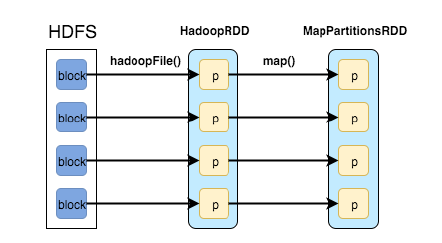
\includegraphics[width=\textwidth]{bilder/Seminartext-img1.png}
\caption{Erstellung RDD aus HDFS} 
\end{figure}
Wir haben im vorigen Abschnitt gesehen, wie Spark für die Verteilung das
Partitionieren (Sharding) vornimmt. Neben der Verteilung, die hier wie
im gesamten Projekt durch Scale-Out erfolgt, muss sich Spark auch um
Ausfalltoleranz kümmern. Durch die hohe Anzahl eingesetzter Rechner
steigt die Ausfallwahrscheinlichkeit stark an. Um die Erkennnung
ausgefallener Rechner kümmert sich der Ressourcenmanager und ebenso für
die Inbetriebnahme von Ersatzrechnern bzw. weiterer Rechner für höhere
Leistung.

Spark braucht allerdings einen Mechanismus, wie die Analyse fortgeführt
wird, wenn einer der Rechner ausgefallen ist. Zwei Dinge sind
beantworten: wie kommt man an die lokal gespeicherten Daten? Sie sind durch
den Ausfall nicht mehr zugreifbar und wie wird die Berechnung mit
diesen Daten fortgesetzt?

Die Antwort bei Spark ist erstaunlich einfach. Dies liegt daran, dass
die RDDs immutable sind. Dadurch kann das RDD nach erstmaliger
Fertigstellung nicht in einer unsauberen (dirty) Zustand kommen.
Mechanismen für ein UNDO teilweise fertiger Operationen sind also nicht
notwendig. Stattdessen wird nur ein REDO benötigt. Und um dieses Redo
geht es bei der sogenannten Data Lineage. \ Die Grundidee ist es, für
die RDDs die Herkunft, also die Entstehungsgeschichte aufzuzeichnen
bzw. im Voraus zu berechnen. Zur Erinnerung: das verloren gegangene RDD
ist durch eine Reihe von Transformationen von anderen RDDs aus den
ursprünglichen Eingabedaten entstanden. Fällt nun ein Knoten aus und
geht damit das RDD verloren, so können in der Lineage-Datenstruktur für
dieses RDD die Eltern-RDDs gefunden werden. Sofern diese noch vorliegen
(z.B. auf einem nicht-ausgefallenem Knoten), wird einfach die
aufgezeichnete Operation mit den Eltern-RDDs wiederholt. Sind diese
Eltern-RDDs ebenfalls nicht mehr vorhanden oder ausgefallen, so wird in
der Kette rekursiv durchgegangen. Am Ende stehen die orginalen
Eingabedaten. Das Konzept geht davon aus, dass diese Daten bereits
redundant vorliegen. Das ist auch der Fall, wenn z.B. HDFS genutzt wird
die Originaldaten hiervon geladen werden.

Diese Idee kann nun durch Checkpoints ergänzt werden. Unter einem
Checkpoint versteht man hier eine persistente Kopie von RDDs in einer
tieferen Lineage-Ebene. So muss bei einem Ausfall nur bis maximal zu
diesem RDD in dem Checkpoint zurückgegangen werden. Je länger die
Geschichte eines RDD ist, desto lohnender kann dieser Vorgang sein.
Dagegen spricht natürlich der erhöhte Speicherverbrauch.

Neben der Betrachtung auf RDD-Ebene lässt sich diese Betrachtung auch
auf Partitionsebene innerhalb des RDDs übertragen. Den eigentlich sind
die RDDs ja über mehrere Rechner verteilt (Scale-Out) und auf dem
Rechner liegen dann Partitionen verschiedener RDDs und meist nicht das
ganze RDD.

\section[Programmiermodell]{\selectlanguage{ngerman}\rmfamily
Programmiermodell}
Spark ist sowohl ein Framework, dass einfache Möglichkeiten für
verteilte Analysen bereitstellt, als auch eine Möglichkeit die so
erzeugten Analysen durchzuführen.

In diesem Abschnitt wird nochmal genauer auf das Programmiermodell
eingegangen. Die Daten werden mittels Scale-Out-Algorithmen verteilt
analysiert. Um möglichst hohe Parallelisierung zu erreichen, werden die
Daten in den meisten Fällen als unabhängig angenommen. Beispiele für
Eingabedaten sind Datenbanktabellen oder csv-Dateien.

Die einzelnen Einträge werden unabhängig voneinander vorverarbeitet.
Dies geschieht im Map-Schritt. Dann werden die Ergebnisse
zusammengefügt. Das passiert im Reduce-Schritt. So weit entspricht das
Vorgehen dem MapReduce-Programmiermodell. Spark erweitert es um einige
Operationen.

Dabei werden zwei Typen unterschieden: Aktionen, die aus einem RDD einen
konventionellen Datentyp, wie int, erzeugen. Der andere Typ sind
Transformationen, die aus RDDs wieder andere RDDs erzeugen. Dabei
werden neue RDDs erzeugt und nicht ursprünglichen RDDs verändert, denn
RDDs sind ja immutable.

Man könnte also von einem TransformAction-Programmiermodell als
Weiterentwicklung des MapReduce-Programmiermodells sprechen.

Zu den Transformationen gehören auch filter und flatMap. MapReduce
erweckt den Eindruck, dass es zumindest im Map-Schritt eine
1:1-Abbildung zwischen Elementen des einen RDDs zu Elementen des neuen
RDDs besteht. Natürlich lassen sich auch Elemente entfernen, die dann
im neuen RDD nicht mehr vorkommen (filter) und neue Elemente erzeugen. Dafür
wird eine Liste dieser Elemente als Transformationsergebnis für ein
Element erzeugt und statt map flatmap aufgerufen. Dabei werden alle
Listenelemente zu eigenen Elementen in dem neuen RDD.

Beispiele für Aktionen sind:

\begin{itemize}
\item count()
\item collect()
\item reduce()
\end{itemize}
Beispiele für Transformationen sind:

\begin{itemize}
\item map()
\item filter()
\item flatMap()
\item sample()
\item join()
\item sort()
\end{itemize}
Hinweis: Zur Zeit stellt Spark seine API von RDDs auf Dataframes um.
Diese haben deutlich erweiterte Möglichkeiten. Sie können mit ähnlichen
Operationen wie die von SQL bearbeitet werden.


\subsection{Beispielcode}

\subsubsection{Bekannte Wordcount}
\lstinputlisting[language=Java]{bilder/wordcount.scala}


\subsubsection{Approximation von PI}
\lstinputlisting[language=Java]{bilder/pi.scala}

Die Funktionsweise ist wie folgt: \ math.random liefert einen Wert
zwischen 0 und 1. Wir stellen uns einen Einheitskreis vor. Sein
Flächeninhalt ist$\pi r^2$, also bei $r=1$ $\pi$. Nun wird geprüft, ob die Koordinate (x,y) in
dem Einheitskreis liegt. Wenn dies der Fall ist, dann wird sie gezählt.
Der Anteil der Koordinaten, die in dem Einheitskreis liegen im
Vergleich zu der Gesamtzahl an Samples, entspricht gerade
$\frac{1}{4}\pi$ Der Faktor Vier
kommt daher, dass wir nur den ersten Quadraten des Einheitskreis
betrachten.

\section[Spark und Distributed Shared
Memory]{\selectlanguage{ngerman}\rmfamily Spark und Distributed Shared
Memory}
Am Anfang haben wir als ein Ziel von Spark die Abstraktion für
Distributed Shared Memory beschrieben. Das wollen wir nun nochmal
aufgreifen und beide vergleichen. Dadurch, dass die Operationen
gegenüber der Distributed Shared Memory eingeschränkt werden, nämlich
insbesondere Veränderungen nur bei gleichzeitiger Kopie des RDDs
vorgenommen werden können, entfallen viele Aufgaben. Distributed Shared
Memory funktioniert wie verteilter Arbeitsspeicher, d.h. die einzelnen
Rechner können mehr oder weniger unreguliert Lese- und
Schreiboperationen vornehmen. Damit das nicht im Chaos endet, müssen
sie sich Protokolle zur Synchronisation nutzen. 

Betrachten wir einige Aufgaben genauer:


\begin{itemize}
\item Konsistenz der Daten sicherstellen
\end{itemize}
Ist bei RDDs nicht notwendig, da die RDDs immutable sind. Es muss nur
überwacht werden, ob das RDD vollständig erzeugt wurde. Dadurch wird der
ganze Transformationsvorgang atomar. Bei Distributed Shared Memory ist
das nicht so. Da sind zusammengehörige Schreiboperationen nicht atomar,
d.h. es ist durchaus möglich, dass der erste Teil der
Schreiboperationen bereits umgesetzt wurde (z.B. Kontostand bei einer
Überweisung verringern), der zweite Teil aber nicht (z.B. Kontostand
beim Empfänger erhöhen). Deshalb muss die Anwendung hier ein spezielles
Protokoll zwischen den Knoten einführen.

\begin{itemize}
\item Fault Recovery
\end{itemize}
Kann bei RDDs durch Lineage vergleichsweise einfach vorgenommen werden.
Bei Distributed Shared Memory ist wieder ein kompliziertes Protokoll
notwendig. Checkpoints sichern die Daten. Da die Konsistenz aber nicht
notwendigerweise gegeben ist, braucht es Rollback-Vorgänge. 

Eindeutiger Nachteil der RDDs ist ihr schlechter Umgang mit
feingranualaren Schreibevorgänge, d.h wenn nur wenige Elemente eines
RDDs geändert werden sollen. Distributed Shared Memory liegt hier
eindeutig vorne, da alle Operationen feingranular erfolgen können.

\section[Spark{}-Architektur]{\selectlanguage{ngerman}\rmfamily
Spark-Architektur}
Hauptaugenmerk in diesem Abschnitt soll auf der Berechnung der Job
Stages liegen. Mit Hilfe der Transformationen und Aktionen lassen sich
komplexe Abfolgen von Operationen auf unterschiedlichen RDDs und auch
in Kombination dieser RDDs erzeugen. Während die Transformationen für
alle Partitionen parallel ausgeführt werden können, müssen die parallel
erfolgenden Operationen durch Spark erst berechnet werden.

Dazu werden die komplexen Operationsfolgen in Stages unterteilt. Sie
entsprechen den Knoten in einem DAG (einem azyklischen Graphen).
Dadurch entsteht eine partielle Ordnung der Stages. Stehen zwei Stages
weder in einer Vor- noch in einer Nacheinander-Beziehung, so können sie
parallel berechnet werden, sofern ihre Eltern-RDDs bereits berechnet
wurden. 

Ein entscheidender Unterschied stellen hier die Operationen da. Sind die
Operationen Joins oder groupByKey, so müssen alle daran beteiligten
RDDs vollständig berechnet sein, damit die Operation ausgeführt werden
kann. Man spricht dann von einer wide dependency. D.h. bei der
Ausführung muss das erste RDD auf die anderen RDDs warten. Andere
Operation wie map, union, join mit co-partitionierten Input oder filter
brauchen das nicht. Sie liegen innerhalb eines Stages in einer Abfolge.
Man spricht hier von narrow dependencies.

\begin{figure}
\centering
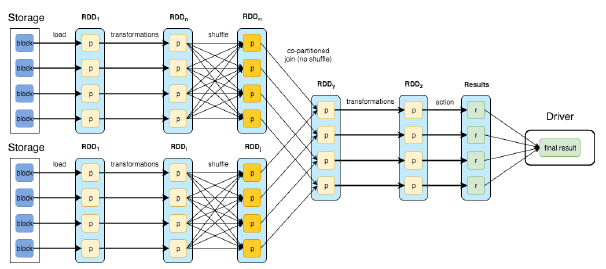
\includegraphics[width=\textwidth]{bilder/Seminartext-img2.png}
\caption{Spark Stages}
\end{figure}

\bigskip

\subsection[Durchlauf durch
Komponenten]{\selectlanguage{ngerman}\rmfamily Durchlauf durch
Komponenten}
Betrachten wir nun Einbindung der Job-Stage-Berechnung in die
Architektur. Alles fängt mit den RDDs an, die inkl. ihrer Lineage aus
dem Javacode ermittelt werden. Sie werden als DAG in den DAGScheduler
eingegeben. Dieser berechnet die möglichen Jobstages und ermittelt
daraus TaskSets für die einzelnen Rechnenknoten. Er gibt sie an den
Clustermanager weiter. Dieser verteilt sie dann an geeignete Knoten. In
diesen Knoten, den Executors, werden diese dann in Threads ausgeführt. 

\begin{figure}
\centering
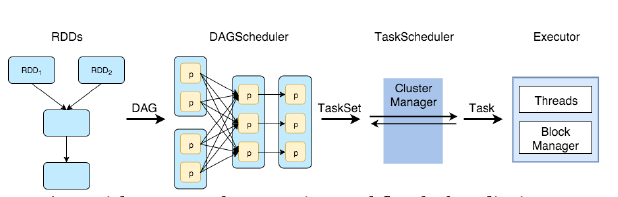
\includegraphics[width=\textwidth]{bilder/Seminartext-img3.png}
\caption{Spark Architektur}
\end{figure}

\bigskip

\section[Vor{}- und Nachteile von
Spark]{\selectlanguage{ngerman}\rmfamily Vor- und Nachteile von Spark}
Fassen wir nochmal die Vorteile und Nachteile von Spark zusammen.
Entscheidend ist die Art von Programm, das ausgeführt werden soll.
Jenachdem ist Spark besser oder weniger gut geeignet.

Schlecht geeignete Programme sind Programme mit vielen asynchronen,
feingranularen Updates auf einem gemeinsamen Zustand. Dies würde zu
einer Explosion der Anzahl von RDDs führen. Beispiele hierfür sind
Web-Anwendungen und inkrementelle Web-Crawler. Alternativen wären
RAMCloud, Percolator und Piccolo.

Gut geeignete Programme führen Bulk Writes auf vielen Daten aus.
Insbesondere dann, wenn Datenlokalität ausgenutzt werden kann, ist
Spark gut geeignet. Spark punktet dann mit effizienter Fault Tolerance
durch Lineage und Ausgleich von langsamen Knoten, da kein Rollback
notwendig ist.

\section[Funktionsweise Spark
Streaming]{\selectlanguage{ngerman}\rmfamily Funktionsweise Spark
Streaming}
Als letztes wollen wir noch die Funktionsweise einer Variante von Spark
anschauen, nämlich Spark Streaming. Wenn man nicht auf periodisch
ausgeführte Analysen warten möchte, sondern gewissermaßen live auf
Ergebnisse zugreifen möchte, kann Spark Streaming eingesetzt werden.

Die Eingabedaten kommen dabei als kontinuierlicher Stream. Sie werden in
Microbatches zerlegt, d.h. es werden z.B. die Daten einer Sekunde
zwischengespeichert. Dann wird ein herkömmlicher Spark-Job auf dem
Batch ausgeführt. Dies wird kontinuierlich für die einkommenden Streams
gemacht. Spark nennt dieses Vorgehen D-Streams. Es ist ein Denkmodell
dafür, dass einkommende Einträge als Microbatches in einem RDD
gespeichert werden. Auf diesem werden dann parallel deterministische
Operationen ausgeführt, analog wie bei der Batch-Analyse. Ein D-Stream
ist also eine Folge von Datensets. Es ist keine komplexe
Synchronisation der einzelnen Knoten notwendig. Sie operieren
unabhängig voneinander und bekommen ihre Aufgaben aus dem DAGScheduler
vorgegeben. Sie greifen nicht auf gemeinsamen Speicher schreibend zu.
\ Ausfälle von Knoten sowie zu langsame Knoten lassen sich genau wie
sonst auch beheben. 

\begin{figure}
\centering
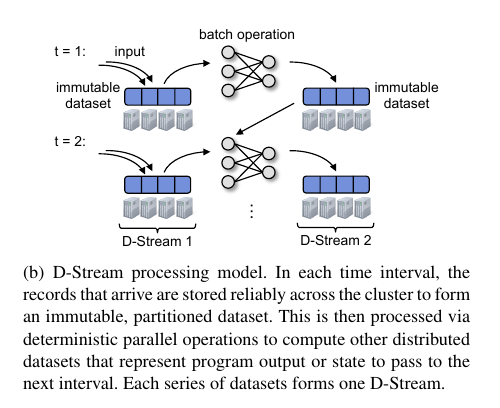
\includegraphics[width=\textwidth]{bilder/Seminartext-img4.png}
\caption{Sparks DStreams}
\end{figure}
\subsection[alternatives, nicht verwendetes
Denkmodell]{\selectlanguage{ngerman}\rmfamily alternatives, nicht
verwendetes Denkmodell}
Ein alternatives Modell wäre der Continuous Operator. Dabei haben die
Nodes einen inneren Zustand, ggfs. gibt es einen dezidierten
gemeinsamen Zustand. Ausfalltoleranz kann dann mit einem
Synchronisationsprotokoll erreicht werden, das Replikation vorsieht.
Schwieriger ist hier die Recovery. Da die zusammenhängenden
Schreiboperationen nicht atomar ausgeführt werden, braucht man wie bei
bei Distributed Shared Memory Rollback und weitere Mechansimen.

Allerdings können hiermit auch komplexere Berechnungen vorgenommen
werden. Es gibt die künstlichen Microbatches-Grenzen nicht.
Dementsprechend sind z.B. Rolling-Windows einfacher. 
	

\chapter{MapReduce}
\label{MapReduce}

\section{Modell}

MapReduce ist ein generalisierter Ansatz für verteile Datenverarbeitung.
Zusätzlich wird mit MapReduce eine Laufzeitumgebung vorgeschlagen, welche für die automatische Verteilung und Parallelierung zuständig ist und außerdem Fehlerbehandlung, sowieso Kommunikation während der verteilten Berechnung abdeckt.
Folgende Übersicht basiert auf dem Paper \textit{MapReduce: Simplified Data Processing on Large Clusters} \cite{mapReduce}.


\begin{figure}[H]
	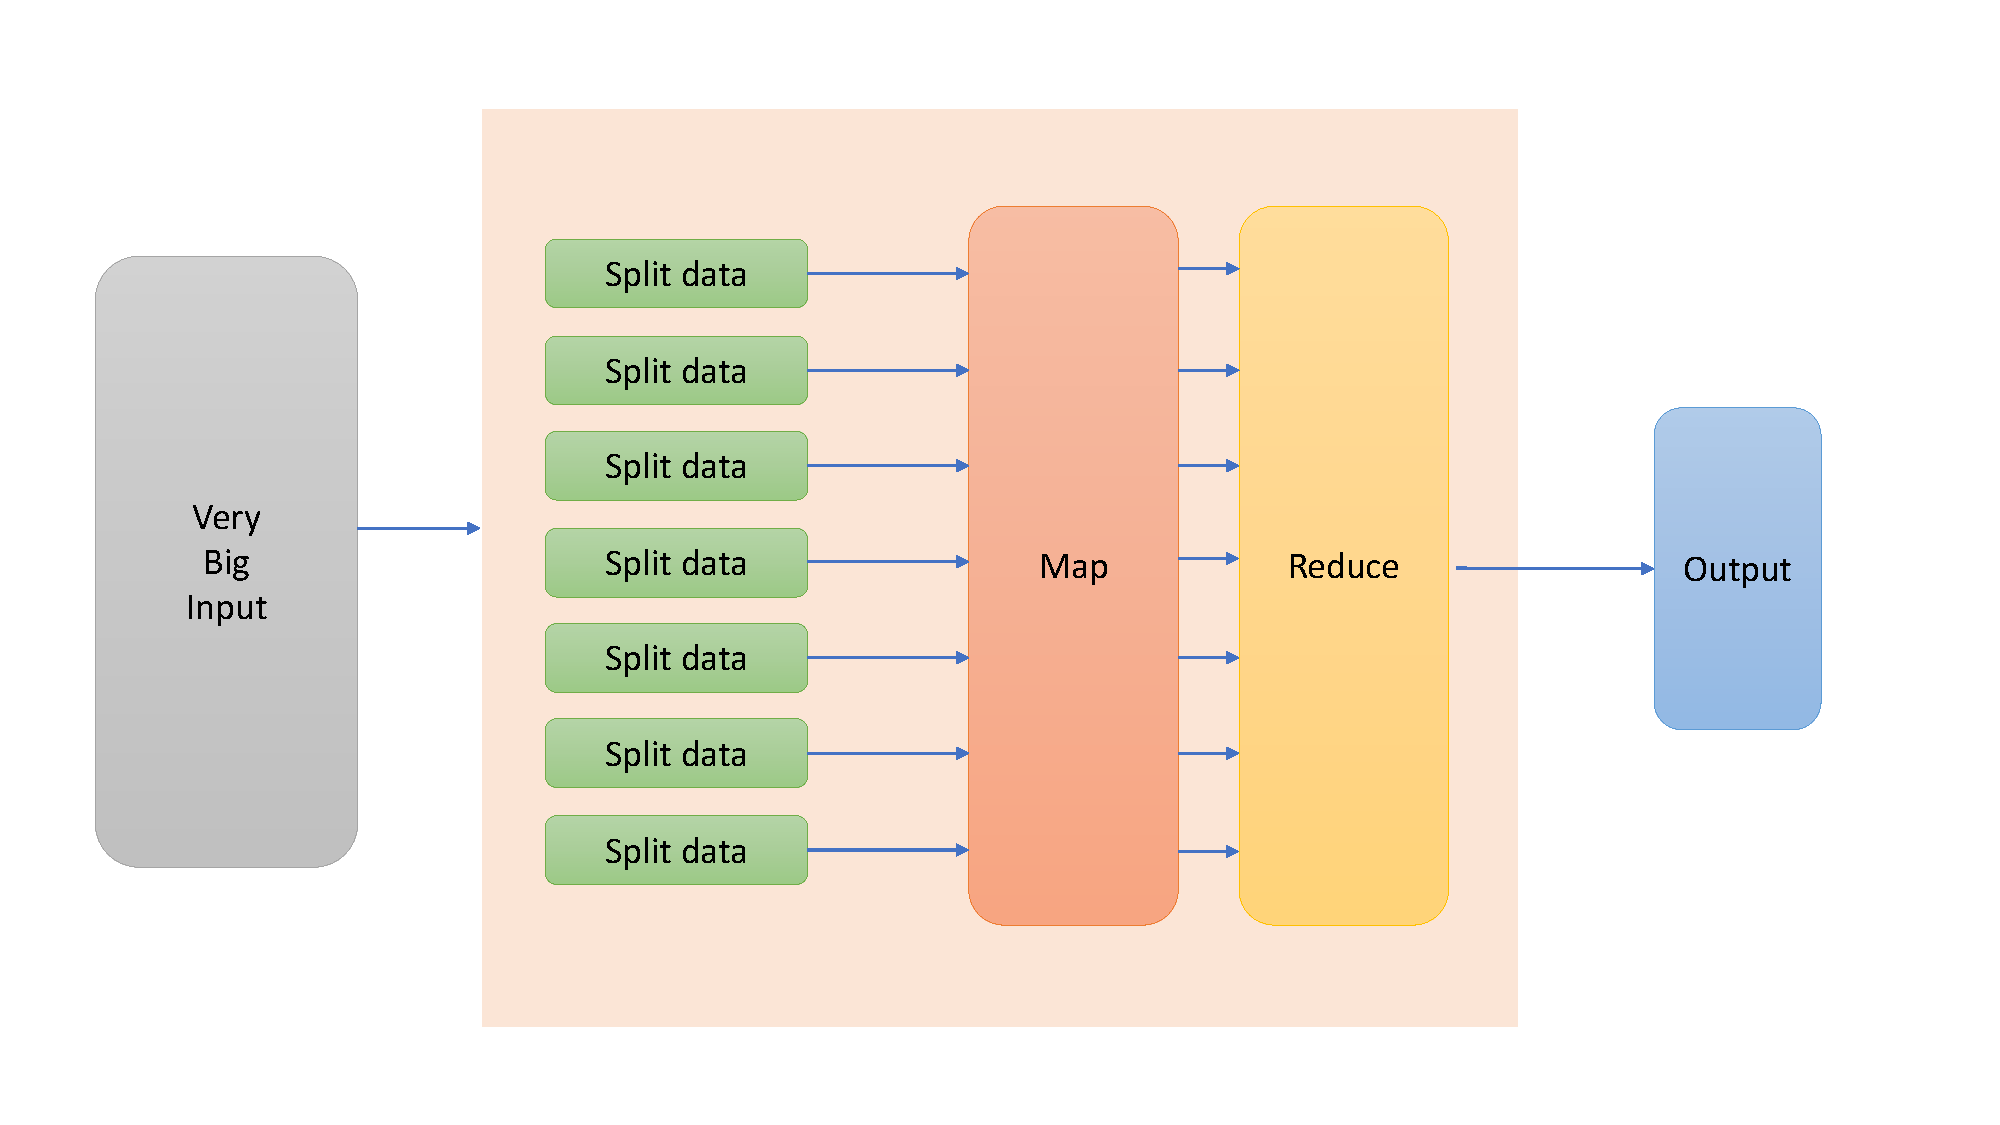
\includegraphics[width=\textwidth]{pics/mapReduce/overview}
	\caption{MapReduce Modell Übersicht}
\end{figure}


Um eine verteilte Berechnung und Verarbeitung zu vereinfachen, wird diese in zwei grobe Phasen aufgeteilt: Map und Reduce.
Für beide Phasen muss der Nutzer jeweils eine entsprechende Funktion definieren.
Der Input liegt als key/value Paare und vor und MapReduce produziert wiederum key/value Paare als Ergebnis.
In der Map Phase werden aus den gegeben key/value Paaren Zwischenwerte berechnet, welche wiederum als key/value Paare vorliegen. Diese werden anschließend gruppiert und in der Reduce Phase weiterbehandelt.
In der Reduce Phase werden dann die berechneten Zwischenwerte für gleiche keys zusammengefasst und aggregiert.

Beispiel:
Für eine Vielzahl von vorliegenden Dokumenten soll die Wortanzahl ermittelt werden.
Dann könnten die Map und Reduce Funktionen wie folgt aussehen:

\begin{lstlisting}[language=json,firstnumber=1]
map(String key, String value):
	// key: document name
	// value: document contents
	for each word w in value:
		EmitIntermediate(w, "1");

reduce(String key, Iterator values):
	// key: a word
	// values: a list of counts
	int result = 0;
	for each v in values:
		result += ParseInt(v);
	Emit(AsString(result));

\end{lstlisting}

Die Map function gibt also einfach jedes Wort plus ein Anzahl, in diesem Falle einfach 1 zurück.
Anschließend würde die Reduce Funktion alle zurückgebenen Anzahlen für jedes Wort summieren.



\section{Implementation}

Für das MapReduce Interface sind laut Paper (cite) verschiedene Umsetzungen möglich, die sich an den  Ausführungsumgebungen ausrichten.
Im Paper wird dann eine Umsetzung für eine damals typisch eingesetzte Environment vorgestellt.
Als Ausführungsumgebungen werden große Cluster (Anzahl 100-1000 Knoten) von Computern mit durchschnittlicher Rechenleistung und Hauptspeicher genannt.
Folgend wird beschrieben wie die Verteilung der Map und Reduce Funktion in dieser Umgebung von Google implementiert wurde.
Aufden Knoten läuft ein verteiltes Dateisystem (GFS), welches ein Zugriff auf Dateien über das Netzwerk ermöglicht, ein Knoten jedoch dabei diese Dateien wie lokate Dateien behandeln kann.
Der Nutzer übermittelt den MapReduce-Job an ein Scheduling System, welches dann die Ausführung koordiniert.


\subsection*{Vorbereitungen}
Ein Knoten übernimmt die Aufgabe des Masters, welcher dann die weitere Ausführung und das Scheduling übernimmt.
Der übermittle MapReduce-Job wird dann wie folgt in verschiedene Tasks aufgeteilt:
\begin{enumerate}
	\item
	Die Eingabedaten werden in M Parts gesplittet, pro Part wird später ein Map-Task ausgeführt.
	\item
	Die Reduce-Phase wird in R Reduce-Tasks aufgeteilt.
	Hierzu wird die Menge der möglichen Zwischenergebnisse
	durch eine Verteilungsfunktion in R Partitionen aufgeteilt.
\end{enumerate}
Diese Tasks werden den Workern dann dymamisch während der Ausführung zugeteilt.
Typische Zahlen sind: Z.B: M=200.000 R=4000, workers=2000

\subsection*{Ausführung der Map Phase}

In der Map Phase teilt der Master jedem freien Worker einen Map-Task zu.
Der Worker liest den zum Map-Task gehörenden Datenpart und führt darauf die Map-Funktion aus.
Hierbei werden (bis zu) R lokale Dateien (eine Datei pro Key) mit
Zwischenergebnissen lokal gespeichert.
Zum Schluss übermittelt der Worker den Speicherort der Zwischenergebnisse an den Master, damit diese später verteilt werden können.

\begin{figure}[H]
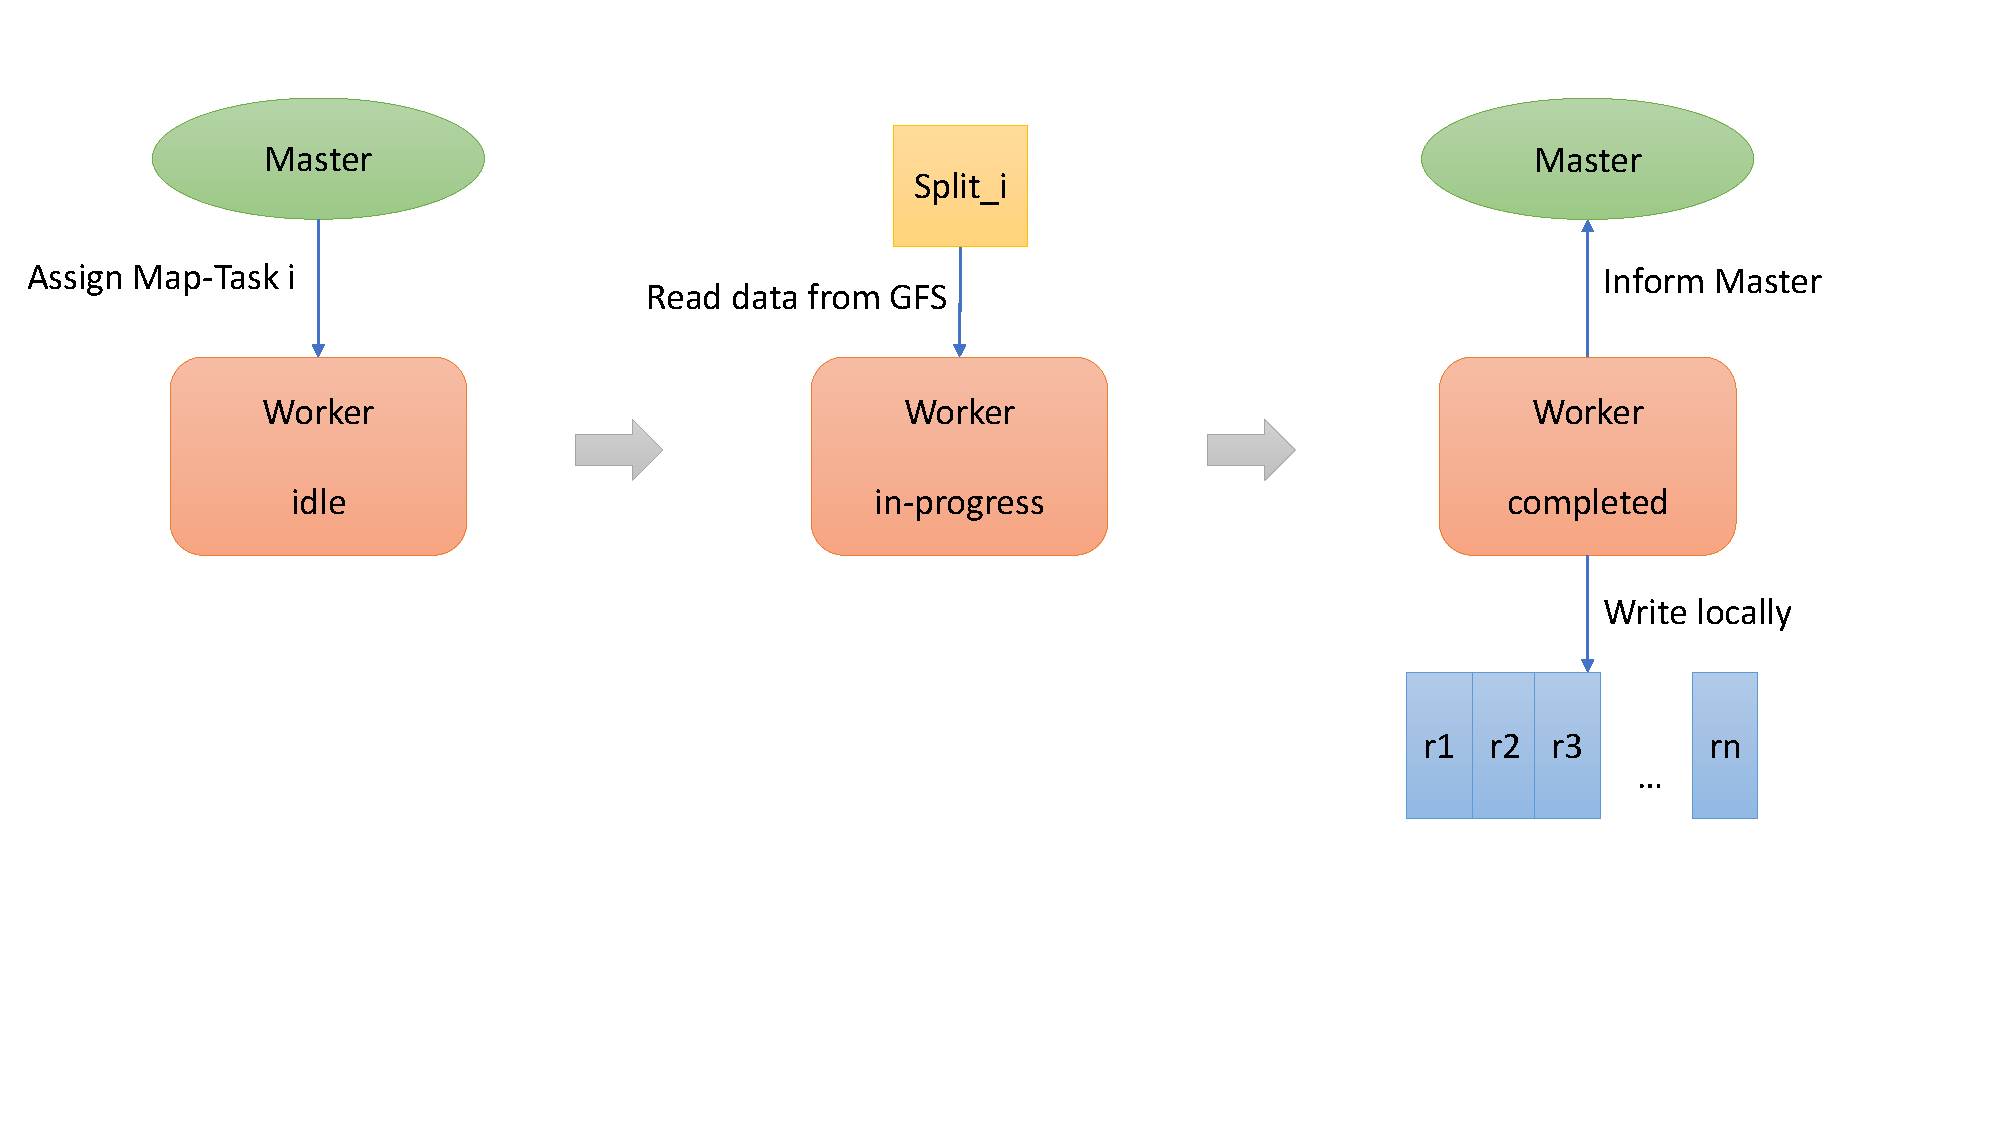
\includegraphics[width=\textwidth]{pics/mapReduce/mapassign}
	\caption{Ausführung eines Map tasks}
\end{figure}

\subsection*{Ausführung der Reduce Phase}

Der Master verteilt die Reduce-Tasks auf freie Worker und übermittelt dabei die Speicherorte der Zwischenergebnisse pro Key.
Dann liest der ausführende Worker die Zwischenergebnisse pro Key mittels RPC von den anderen Knoten, sortiert die Daten und wendet die vom User definierte Reduce-Funktion darauf an.
Anschließend wird ein Output-File mit dem Ergebnis ins verteilte Dateisystem geschrieben.


\begin{figure}[H]
	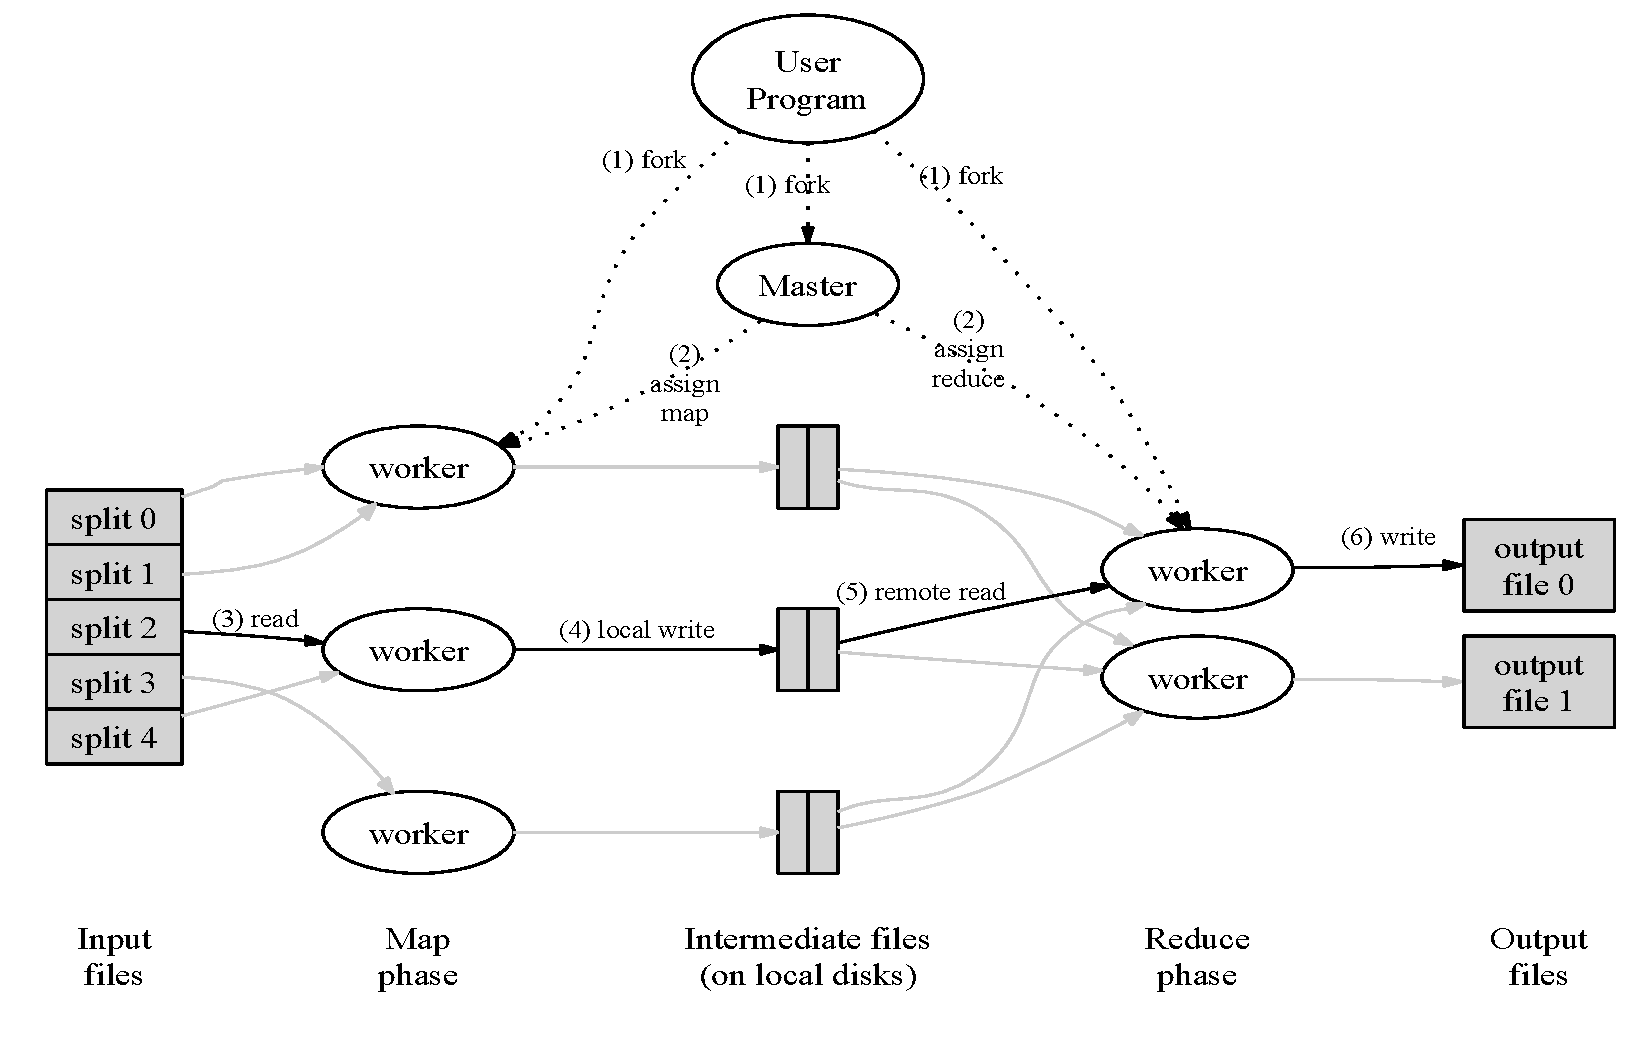
\includegraphics[width=\textwidth]{pics/mapReduce/mapreduce-osdi04e}
	\caption{Übersicht der gesament MapReduce Ausführungslogik}
\end{figure}


\subsection*{Fehlertoleranz}

Da MapReduce für den parallel Einsatzu auf vielen Knoten gedacht ist und einzelne Knoten ausfallen können, gibt es spezielle Fehlerfälle die betrachtet und behandelt werden.

Um ein Failure des Masterknotens aufzufangen, schreibt dieser periodisch Checkpoints vom derzeitigen Ausführungsstatus.
Tritt nun ein Fehler im Master auf, wird ein neuer Knoten als Master gestartet und die Ausführung vom letzten Checkpoint fortgeführt.

Jeder Workerknoten wird vom Master mittels Heartbeat periodisch auf Erreichbarkeit und Status abgefragt.
Wird ein ausgefallener Worker oder ein fehlerhafter Job erkannt, wird zwischen abgeschlossenen und nicht abgeschlossenen Job unterschieden.
Ein nicht abgeschlossener Map oder Reduce Task wird einfach auf einem anderen Worker neu gestartet.
Abgeschlossene Map Tasks werden auch erneut ausgeführt, da die Zwischenergebnisse lokal auf den Knoten liegen und diese entsprechend fehlen.
Abgeschlossene Reduce Tasks müssen nicht erneut ausgeführt werden, weil die Ergebnisse im verteilten Dateisystem gespeichert werden.


\section{Refinements}

Zur eigentlichen Ausführungslogik gibt es noch weitere Refinements, die die Ausführung optimieren.
\subsection*{Combiner}
In der Map Phase entstehen oftmals Wiederholungen von Zwischenergebnissen.
Im Wordcount Beispiel:
\begin{verbatim}
(foo bar bar bar) → (foo, 1) (bar, 1) (bar, 1) (bar, 1)
\end{verbatim}

Ein Worker kann nach Abschluss einen Map-Tasks die Zwischenergebnissen pro key mittels Combine Funktion zusammenfassen.
Z.B.
\begin{verbatim}
(foo, 1) (bar, 1) (bar, 1) (bar, 1) → (foo, 1) (bar, 3)
\end{verbatim}


\subsection*{Partitioning Function}

Die Nummer der Reduce-Tasks wird von Nutzer festgelegt.
Nun gibt es eine default Partitioning Function (hash(key) mod R),
welche die Zwischenergebnisse nach Keys den Reduce-Tasks zuordnet.
Durch die default PF werden meist gut verteilte Partitionen generiert,
allerdings kann der Nutzer auch eigene Verteilungsfunktionen definieren.

\subsection*{Datenlokalität}

Die Inputdaten werden im verteilten Dateisystem in Blöcke geteilt und repliziert auf verschiedenen Knoten gespeichert.
Da diese Blöcke später den MAP-Tasks zugeordnet sind, versucht der Master die Tasks so zu verteilen, dass die benötigten Blöcke auf den zugeordneten Knoten oder zumindest physisch in der Nähe liegen.
Hierdurch wird der Netzwerkdurchsatz während der Taskausführung reduziert und eine Ausbremsung verhindert.


\subsection*{Backup Tasks}

Einzelne, aufgrund Nebeneffekten sehr langsame Knoten, können den Gesamtprozess aufhalten, besonders wenn diese zum Ende eine Phase auftreten.
Um dies zu vermeiden, werden zum Ende einer MapReduce Phase Tasks welche noch nicht abgeschlossen sind, repliziert und auf mehren Knoten parallel ausgeführt.
Der erste abgeschlossene Task 'gewinnt' und langsame Knoten werden übergangen.


\section{Probleme und Nachteile von MapReduce}

MapReduce udn Spark (siehe chapter spark) ermöglichen die parallele und verteile Verarbeitung von riesigen Datenmengen.
Allerdings speichert und verarbeitet MapReduce alle Daten auf der Platte, während Spark durch eine in-memory Verarbeitung bis zu 100 mal schneller ist.
Auch bei iterativer Verarbeitung kann Spark durch die RDDs mehrere Operationen im Speicher ausführen, 
während MapReduce für jede Iterationen einen gesamten Durchlauf anstößt.
MapReduce zwingt den Nutzer die Verabeitung der Daten in eine Map- und eine Reduce-Funktion aufzuteilen, Spark bietet dem Nutzer hier viel mehr Komfort, weil zusätzliche Operationen möglich sind und eine High Level API anbietet. 

Zusätzlich bietet Spark eine Möglichkeit Streams zu verabeiten, was gerade in Hinsicht auf unseren Anwendungsfall, nämlich die Verarbeitung und live Analyse von Twitterdaten interessant ist. 


	\colorlet{punct}{red!60!black}
\definecolor{background}{HTML}{EEEEEE}
\definecolor{delim}{RGB}{20,105,176}
\colorlet{numb}{magenta!60!black}

\lstdefinelanguage{json}{
    basicstyle=\normalfont\ttfamily,
    numbers=left,
    numberstyle=\scriptsize,
    stepnumber=1,
    numbersep=8pt,
    showstringspaces=false,
    breaklines=true,
    frame=lines,
    backgroundcolor=\color{background},
    literate=
      {0}{{{\color{numb}0}}}{1}
      {1}{{{\color{numb}1}}}{1}
      {2}{{{\color{numb}2}}}{1}
      {3}{{{\color{numb}3}}}{1}
      {4}{{{\color{numb}4}}}{1}
      {5}{{{\color{numb}5}}}{1}
      {6}{{{\color{numb}6}}}{1}
      {7}{{{\color{numb}7}}}{1}
      {8}{{{\color{numb}8}}}{1}
      {9}{{{\color{numb}9}}}{1}
      {:}{{{\color{punct}{:}}}}{1}
      {,}{{{\color{punct}{,}}}}{1}
      {\{}{{{\color{delim}{\{}}}}{1}
      {\}}{{{\color{delim}{\}}}}}{1}
      {[}{{{\color{delim}{[}}}}{1}
      {]}{{{\color{delim}{]}}}}{1},
}

\chapter{Search Engine}
Die Twitter-Klon Applikation soll mit einer Suchfunktion erweitert werden. Diese Suchfunktion wird mit einem Such-Service umgesetzt, der auf der Elasticsearch-Engine basiert. Elasticsearch setzt auf Apache Lucene auf, einer in Java geschriebenen Bibliothek für die Volltextsuche. Es ist open-source, dokumentenorientiert, in Java geschrieben und lässt sich über einen REST-API ansprechen. Damit ist es ein guter Kandidat für unser Use-Case.

\section{Zielsetzung}
Das Ziel des Suchservices ist die Ausgabe von \textit{best-match} Ranglisten über eine Tweets-Sammlung zu erstellen, indem man nach bestimmten Benutzern, Tags und Freitexteingaben sucht. Als Erweiterung der Suchfunktion wird ein Text-Vervollständigung Feature erstellt, das beim Suchen nach Tweets passende Vorschläge liefert. Und zum Schluss sollen ausgewählte Datensätze, mit Hilfe eines Analyse- und Visualisierungstools, auf der Homepage als eine Grafik angezeigt werden. 

\section{Vorgehen}
Zuerst wird eine \textit{Elasticsearch-Service} Architektur angefertigt. Diese stellt nur ein Teil der \textit{Twitter-Klon} Umsetzung und behandelt die Kommunikation zwischen \textit{Elasticsearch}, \textit{Elasticsearch-Service} wie den \textit{Kafka-Topics}. Nachfolgend wird Elasticsearch entsprechend der \textit{Twitter-Klone} Applikation konfiguriert und für die Datenaufnahmen vorbereitet. Infolgedessen wird der Such-Service implementiert, der \textit{Elasticsearch} mit den \textit{Kafka-Topics} verbindet und für den Datenaustausch zuständig ist. Anschließend werden Datenvisualisierungen mit Hilfe von \textit{Kibana} angefertigt. Zum Schluss wird der Elasticsearch Abschnitt mit einem Fazit beendet.

\section{Service Design}
Der komplette Nachrichtenaustauch der \textit{Twitter-Klon} Applikation wird mit einem skalierbaren und performanten Messaging-Service umgesetzt, nämlich \textit{Apache Kafka}. Dieser, bietet die Möglichkeit, mit Hilfe der Nachrichten-Topics den Overhead an Kommunikation zwischen den Services zu verringern, die Services von einander zu entkoppeln und die Daten parallel zu verarbeiten.
Diese Eigenschaft ermöglicht das Entkoppeln des Such-Service‘es von dem Restsystem, sodass die Suche unabhängig von den Schnittstellen der heterogenen Klienten bedient werden kann. 
Dafür wurden drei Topics erstellt und ein Datenformat vereinbart, das langfristig alle unsere Wünsche abdecken soll. Die Such-Service Use-Cases sind in drei Gruppen eingeteilt, die mit Hilfe von drei Kafka-Topics realisiert wurden: Neue Dokumente indexieren/abspeichern, Anfragen empfangen und Anfragen beantworten.
%\captionsetup{justification = raggedright,singlelinecheck = false}
\begin{figure}[htbp!]
	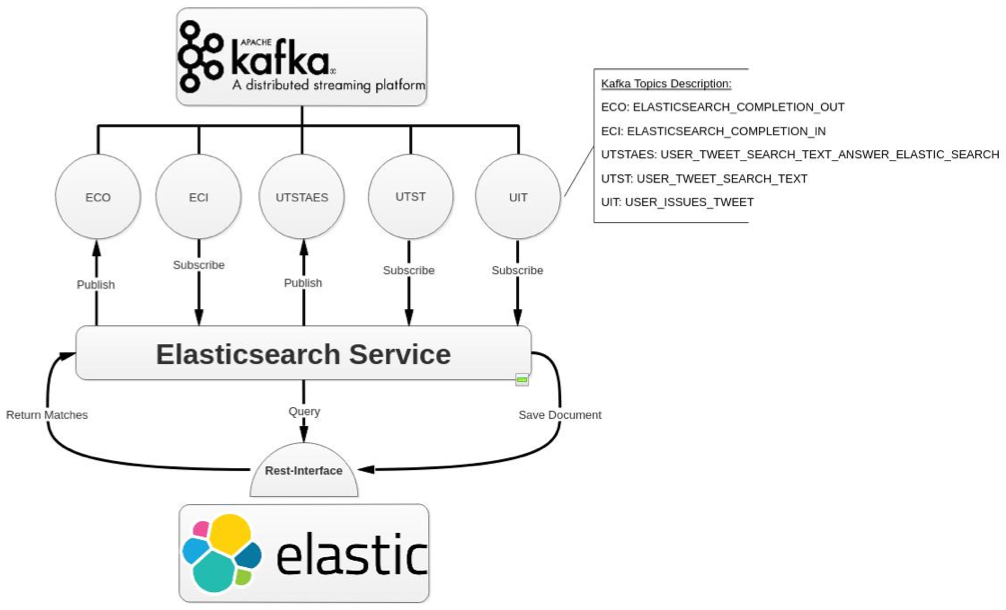
\includegraphics[scale=0.8]{material/architecture/Elasticsearch.png}
	\caption{Elasticsearch Service Architectur}
	\label{fig:ESA}
\end{figure}

Der Such-Service meldet sich an den entsprechenden Kafka-Topics an, öffnet ein Datenstrom und empfängt Nachrichten mit den Speicher-, Suchkriterien, sowie der dazugehörigen Benutzerkennung. Um den Speicherplatz optimal zu nutzen, werden aus der Nachricht nur für die Suche relevante Felder ausgelesen und an die Elasticsearch REST-Schnittstelle weitergeleitet, wie z.B. der Text, die Benutzerkennung, die Tags und der Zeitstempel.  

Das Verschicken der Nachrichten über unsere Applikation durchläuft den \textit{UIT} Topic, dieser bietet jedem Abonnenten den Zugriff auf die neu eingetroffenen Mitteilungen. Der Elasticsearch-Suchservice ist einer der bestehenden Abonnenten des \textit{UIT} Topics und bereitet die neu eingetroffenen Nachrichten für die Weiterleitung und das Speichern des Inhalts in Elasticsearch. Die, mit Metainformation bestückten, Nachrichten laufen eine Transformation durch wie Filterung, Umbenennung und Umstrukturierung, um der Elasticsearch erwarteten Datenstruktur zu entsprechen und Speicherplatz zu sparen. 

Für die Suchfunktion werden die Topics \textit{UTST} und \textit{UTSTAES} genutzt. Über den \textit{UTST} werden Suchanfragen entgegengenommen und in eine Elasticsearch-Rest-Anfrage umgeformt. Die Suchanfrage kann von dem Suchservice auf verschiedene Weise durchgeführt werden. Zum Beispiel durch eine Term-, Bollean-, Match-, Multimatch- und Match-Phrase- Suche. Jede Abfrageart, kann im bestimmten Fällen vorteilhaft ausgenutzt werden und kann Fallspezifisch eingesetzt werden. 
Das Suchergebnis wird anschließend als eine sortierte Identifikationsliste zu enthaltenen Nachrichten auf dem \textit{UTSTAES} Topic hinterlegt. Damit wäre die Suche beendet und das weitere Geschehen des Suchergebnisses den \textit{UTSTAES} Abonnenten überlassen.

Die Suchvervollständigung verhält sich ähnlich der Suchfunktion. Der Suchservice kommuniziert über die Topics \textit{ECI} und \textit{ECO}, die vervollständigung Anfragen für die Benutzereingabe publizieren und mögliche Eingabewünsche entgegennehmen. Die Eingabewünsche könne mit Hilfe der Elasticsearch Vervollständigung oder durch die nGrams-Implementation umgesetzt werden. Diese Ansätze sind in der Granularität, Umsetzung, Laufzeit und Speicherbedarf unterschiedlich und könne Fallabhängig ausgetauscht werden. 


\section{Elasticsearch Konfiguration}
Elasticsearch funktioniert \textit{out of the box}, das heißt, man muss den Service nur starten und das Indexieren, wie das Suchen der Dokumente funktioniert reibungslos. Im Gegensatz zu den relationalen Datenbanken ist eine Schema Definition für Elasticsearch nicht notwendig. Obwohl ein Schema nicht gefordert ist, ist es höchst ratsam dieses zu deferieren, denn das \textit{Type-Matching} der Felder wird ansonsten nach dem \textit{Best Guess} Prinzip erstellt und kann unter umstanden zum unerwünschten Verhalten führen.

\subsection{Index Settings}
Die \textit{out of the box} Fähigkeit von Elasticsearch ist toll zum Ausprobieren, jedoch ist es für den Betrieb ungeeignet, da die Einstellungen für die bestmögliche Skalierung von Elasticsearch, wie das Durchsuchen der Texte immer von der Domäne abhängt. Falsche oder keine Anpassung, kann die Skalierungsmöglichkeiten von Elasticsearch drastisch senken und damit den Betrieb unerwartet unterbrechen. Des Weiteren ist die Anpassung der Textvorverarbeitung eine Kernaufgabe jeder Such-Engine, dementsprechend sollte man sich besonders sorgfältig um diese Aufgabe kümmern, sodass alle relevanten Ergebnisse ermittelt und in einer passenden Ordnung dem Nutzer vorgelegt werden können.

\subsection{Sharding \& Replication}
Zuerst wird der Elasticsearch Index auf Shards und Replicas aufgeteilt. Damit enthält ein Shard eine Teilinformation oder ein Replikat der Teilinformation des Indexes, der auf unterschiedliche Hardware aufgeteilt werden kann. Obwohl die Verschiebung des Shards Knotenübergreifend realisiert werden kann, kann dieser nicht in zwei neue Shards gespalten werden, wenn die Hardware an ihre Grenzen stößt. Damit ist ein Shard die Skalierungseinheit des Indexes und muss sorgfältig gewählt werden. Der uns gegebene Elasticsearch Cluster arbeitet nur auf einem Knoten, dementsprechend ist der Skalierungsfaktor von fünf genug um zukunftssicher den Index bis auf fünf weitere Knoten aufteilen zu können. Der Replikationsfaktor beschreibt wie viele Replikate für einen Shard erstellt werden. Für eine Einstellung aus fünf Shards und einem Replikat entsteht eine Gesamtdatenmenge von 10 Shards. Daraus folgt ein immenser Anstieg an Speicherverbrauch für jeden nächsten Replikat eines Shardes. Die Replikate bieten im Gegensatz die Ausfallsicherheit und die Performance Steigerung der Lesezugriffe. Da die Performance und die Ausfallsicherheit für jeder skalierbare Applikation Kernkriterien sind, kann Elasticsearch diese bei Bedarf im laufenden Betrieb durch neue Replikate stärken. In unserem Fall steht nur einen Knoten zur Verfügung, dementsprechend folgt kein Anstieg der Performance wie Ausfallsicherheit mit Hilfe der Replikation.
% Bild  mit Reploikation der Shards und Replikas auf Knoten.
\\\\
\textbf{Initiale Index Einstellungen}
\begin{lstlisting}[language=json,firstnumber=1]
{
  "twitterindex": {
    "settings": {
      "index": {
        "number_of_shards": "2",
        "number_of_replicas": "0",
        "refresh_interval": "1s",
        "provided_name": "twitterindex",
        "creation_date": "1529674155106",
        ...
        "uuid": "wOHQnu5GQjOs7iP-Cv-_MQ",
        "version": {
          "created": "6020399"
        }
      }
    }
  }
}
\end{lstlisting}

\subsection{Textvorverarbeitung}
Als nächstes wird der Textvorverarbeitungsprozess definiert. Unter dem Schlüssel \textit{Analyzer} wird ein \textit{Custom Analyzer} und die dazugehörigen Vorverarbeitungsschritte erstellt. Dieser wird innerhalb Elasticsearch aufbewahrt und mit Funktionalität belegt. Der Analyzer zerlegt den Text mit dem \textit{Partial Word Tokenizer} in Tokens nach einem bestimmten Muster, nämlich nach einem Leerzeichen, nach einem Großbuchstaben Anfang und nach einer Zahl.
Dieser Zerlegungsschritt erfüllt die gegebenen Anforderungen, könnte aber auf Kosten des Speicherplatzes durch den mächtigeren \textit{Edge NGram Tokenizer} ausgetauscht werden. Nachfolgend laufen die Tokens eine Transformationskette durch. Zuerst werden die Tokens in Kleinbuchstaben umgewandelt, auf den Wortstamm zurückgeführt und Worte mit geringen Informationsgehalt, sowie verboten Worte entfernt. Zuletzt werden die Worte mit ähnlicher Bedeutung wie \textit{Universität Hamburg} und \textit{UHH} in Synonymlisten zusammengefasst und als gleichgültig behandelt. 
\\\\
\textbf{Analyzer}
\begin{lstlisting}[language=json,firstnumber=1]
"analyzer": {
...
  "my_analyzer": {
    "filter": [
      "my_tokenizer",
      "lowercase",
      "my_stemmer",
      "english_possessive_stemmer",
      "my_stop",
      "my_synonym"
    ],
    "type": "custom",
    "tokenizer": "standard"
  },
...
}
\end{lstlisting}

\subsection{Data Mapping}
Zuletzt braucht Elasticsearch ein Datenschema, um die automatische Fehleinschätzung des Mappings zu vermeiden. 
Elasticsearch baut einen Suchindex auf, der Dokumentenbasiert in einem JSON Format abgespeichert wird. Das Mapping garantiert eine Typenzusicherung wie das Format, der zu speichernden Felder und Dokumente. Zum Beispiel das Datumformat, das Regionsunabhängig vor dem Abspeichern von Elasticsearch normalisiert wird oder das Textfeld, das man mit bestimmten Eigenschaften und Funktionen anreichert, um das gewünschte Verhalten zu realisieren. 
Der Text, kann als \textit{Keyword} abgespeichert werden, das Eins-zu-eins durchsucht wird oder ein \textit{Text}, das mit Hilfe der Volltextsuche komplexen Suchkriterien umsetzen kann.
Das Elasticsearch Mapping für den Twitter-Klon definiert ein Dokumentenformat mit sieben Felder: id, message, tags, users, timeStamp, userLocation und userLocationCompletion. Für die Suche sind die Felder \textit{message}, \textit{tags} und \textit{use} relevant, diese werden vom Type \textit{Keyword} und \textit{Text} gespeichert. Das Feld \textit{timeStamp} wird auf ein \textit{Long} projiziert und für die Datenvisualisierung mit Kibana genutzt, um die wöchentlichen Trends anzuzeigen. Das Feld \textit{userLocation} hält die vom Benutzer eingetragene Standort, der mit der Textvervollständigungsinformation von Elasticsearch angereichert und durch das Feld \textit{userLocationCompletion} beschrieben. Zum Vergleich wird das Feld \textit{userLocation}  zusätzlich mit dem \textit{nGram Analyzer} belegt, um die Text-Verfollständigung von Elasticsearch mit der \textit{nGram} Methode vergleichen zu können.  
\\\\
\textbf{Mapping}
\begin{lstlisting}[language=json,firstnumber=1]
"userLocation": {
  "type": "text",
  "analyzer": "nGram_analyzer",
  "search_analyzer": "nGram_search_analyzer"
},
"userLocationCompletion": {
  "type": "completion",
  "analyzer": "simple",
  "preserve_separators": true,
  "preserve_position_increments": true,
  "max_input_length": 50
},
\end{lstlisting}


\section{Search Service}
Die Implementation des Such Service wird mit Java und Spring realisiert. Spring ist ein weit verbreitetes und etabliertes Enterprise Framework für Java. Dieses besitz eine große Palette an Werkzeigen, die das Arbeiten in einer heterogenen Umgebung stark vereinfachen. Daher eignet sich Spring besonders gut für unseren Anwendungsfall. Für den Nachrichtenaustausch zwischen Apache Kafka, Elasticsearch und dem Suchservice wird, die von Spring entwickelte \textit{Spring for Apache Kafka} und die von Elasticsearch angebotene \textit{Elasticsaerch Rest Client} Bibliotheken genutzt.
Die interne Logik des Suchservices wird von den Java Beans umgesetzt, die im Springkontext auf dem Apache Tomcat Application Server ausgeführt werden und die gewünschte Such-Funktionalität umsetzen.

\subsection{Such-Interface}
Um die Kommunikation und Fähigkeiten des Such Services übersichtlich zu gestalten, wird ein Interface mit den gewünschten Anfragen erstellt und anschließend implementiert. 

\begin{enumerate}
	\item über die Tags
	\item über die referenzierten Benutzer
	\item über angegebenen Standortnamen mit der Textvervollständigung
	\item über die Term-Suche auf den Tweet-Text
	\item über die Volltextsuche auf den Tweet-Text
	\item über den Text wie den Benutzet Standortnamen
	\item über einen Zeitraum
	\item über einen Zeitraum mit Benutzer und Tag Präferenz 
\end{enumerate}

\subsection{Such-Implementation}
Elasticsearch bietet eine JSON-ähnliche domänenspezifische Sprache, mit der man Abfragen ausführen kann. Dies wird als \textit{DSL Query} bezeichnet. Die Abfragesprache ist ziemlich umfassend und bietet komplexe Filter und Aggregation Möglichkeiten. Die Anfragen des Suchservices sind ausgelegt die wichtigsten Anfragemöglichkeiten von Elasticsearch darzustellen. Es werden \textit{term}, \textit{match}, \textit{multi match}, \textit{match phrase}, \textit{bool}, \textit{compleation} und \textit{aggregation} Anfragen behandelt. 
\\\\
\textbf{Suchen nach Tags}
\begin{lstlisting}[language=json,firstnumber=1]
{
  "query": {
    "terms": {
      "tags.keyword": "?"
         }
    }
}
\end{lstlisting}

\textbf{Suche nach Referenzierten Benutzer}
\begin{lstlisting}[language=json,firstnumber=1]
{
  "query": {
    "terms": {
      "users.keyword": "?"
    }
  }
}
\end{lstlisting}

Die Tag- und Benutzersuche wird mit der Term-Suche umgesetzt, diese sucht nach Dokumenten, die genau, die im angegebenen Feld angegebenen Begriffe enthalten. Die Tweets werden entsprechend den TF/IDF Relevanz sortiert und präsentiert.  
\\\\
\textbf{Textvervollständigung nach Standortnamen}
\begin{lstlisting}[language=json,firstnumber=1]
{
  "suggest": {
    "location_suggest": {
      "prefix": "?",
      "completion": {
        "field": "userLocationCompletion",
        "fuzzy": {
          "fuzziness": 1
        }
      }
    }
  }
}
\end{lstlisting}
Der Textvervollständigung bietet Funktionen zur automatischen Vervollständigung. Es werden Vorschläge wehrend des Tippens einer Anfrage getätigt und führt schneller zu relevanten Ergebnissen. Durch die zusätzliche \textit{fuzzy} Eigenschaft der Abfrage werden zusätzlich Tippfehler abgefangen um die Suche den Nutzer angenehmer zu gestalten.
\\\\
\textbf{Term-Suche auf den Tweet-Text}
\begin{lstlisting}[language=json,firstnumber=1]
{
  "query": {
    "match": {
      "message": "?"
    }
  }
}
\end{lstlisting}

\textbf{Volltextsuche auf den Tweet-Text}
\begin{lstlisting}[language=json,firstnumber=1]
{
  "query": {
    "match_phrase": {
      "message": {
        "query": "?",
        "slop": 1
      }
    }
  }
}
\end{lstlisting}

Die Suche über den Textkörper eines Tweets kann auf zwei Arten getan werden. Im ersten Fall wird eine Match-Suche \textit{metch} durchgeführt, diese normalisiert die Suchterme, verknüpft sie mit \textit{OR} und durchsucht den Textkörper nach Suchbegriff-Treffern. Im zweiten Fall nutzt man die zusammenhängende Suchanfrage \textit{phrase match}, welche im Gegensatz zu \textit{match} die Terme mit \textit{AND} verknüpft und eine Einschränkungen mitbringt, nämlich die Ordnung der Suchterme im Textkörper. Um die Suche flexibler zu gestalten, kann sie aufgeweicht werden, indem man die akzeptable Entfernung der Suchterme mit der \textit{Slope} Eingeschalt beeinflusst. In unseren Fall erlaubt diese eine Entfernung von einem Wort zwischen den Suchbegriffen.
\\\\
\textbf{Standortabhängige Tweets}
 \begin{lstlisting}[language=json,firstnumber=1]
 {
  "query": {
    "multi_match": {
      "query": "?",
      "fields": [
        "message",
        "userLocation"
      ]
    }
  }
}
\end{lstlisting}
\\\\
Die \textit{multi match} Abfrage sucht nach Nachrichten, dessen Inhalt einen Ort verweist und der Autor sich in dieser Region befindet. Diese Abfrage verhält sich wie \textit{match}, jedoch über eine Menge von Feldern.
\\\\
\textbf{Suche Tweets über den Zeitraum mit referenzierte Benutzer zuerst}
 \begin{lstlisting}[language=json,firstnumber=1]
{
  "query": {
    "bool": {
      "must": {
        "terms": {
          "tags": "?"
        }
      },
      "filter": {
        "range": {
          "timeStamp": {
            "gte": "now-1d/d",
            "lt": "now/d"
          }
        }
      },
      "should": [
        {
          "term": {
            "users": "?"
          }
        }
      ]
    }
  }
}
\end{lstlisting}
Diese Suchanfrage führt ein neues Konzept der \textit{bool} Anfrage, die aus mehreren Komponenten besteht. Die Suche besteht aus erforderlichen Feld-Treffern wie den optionalen Feld-Treffern. Daraus ergibt sich eine Rangordnung aus den relevanten Ergebnissen. Zuletzt läuft die Liste einen Zeitfilter durch um den Zeitraum einzuschränken. 
\\\\
\textbf{Top Tweets für die letzten sieben Tage }
 \begin{lstlisting}[language=json,firstnumber=1]
{
  "aggs": {
    "top_tags": {
      "significant_terms": {
        "field": "tags",
        "size": 10
      }
    }
  },
  "query": {
    "bool": {
      "must": [
        {
          "match_all": {}
        },
        {
          "range": {
            "timeStamp": {
              "gte": "now-7d/d",
              "lt": "now/d"
            }
          }
        }
      ]
    }
  }
}
\end{lstlisting}
Diese Anfrage ist zuständig für die Visualisierung in Kibana. In diesem Fall wird mit Hilfe der \textit{bool} Anfrage und der Elasticsearch-Aggregation, die am häufigsten verwendeten Tag über den Datensatz von sieben Tagen erarbeitet.  
\\\\
\section{Visualisierung mit Kibana}
Die Visualisierungsmöglichkeiten von Kibana sollen es ermöglichen große Datenmengen zu analysieren unterstützt durch flexible Filter. Es bietet Echtzeit-Analyse von Daten, individuell konfigurierbare Visualisierung, dynamische Dashboards und Browserbasiertes Interface, das Plattformunabhängige funktioniert.\\\\
Die Kibana Visualisierungen basieren auf den Aggregationsmöglichkeiten von Elasticsearch. Dieses aggregiert über den Elasticsearch Indexinhalt und erstellt Grafiken, die in HTML eingebunden werden können. Zur Verfügung stehende Visualisierungstypen: Area Chart, Data Table, Line Chart, Markdown Widget, Mertric, Pie Chart, Tile Map, Vertical Bar Chart.
%\captionsetup{justification = raggedright,singlelinecheck = false}
\begin{figure}[htbp!]
  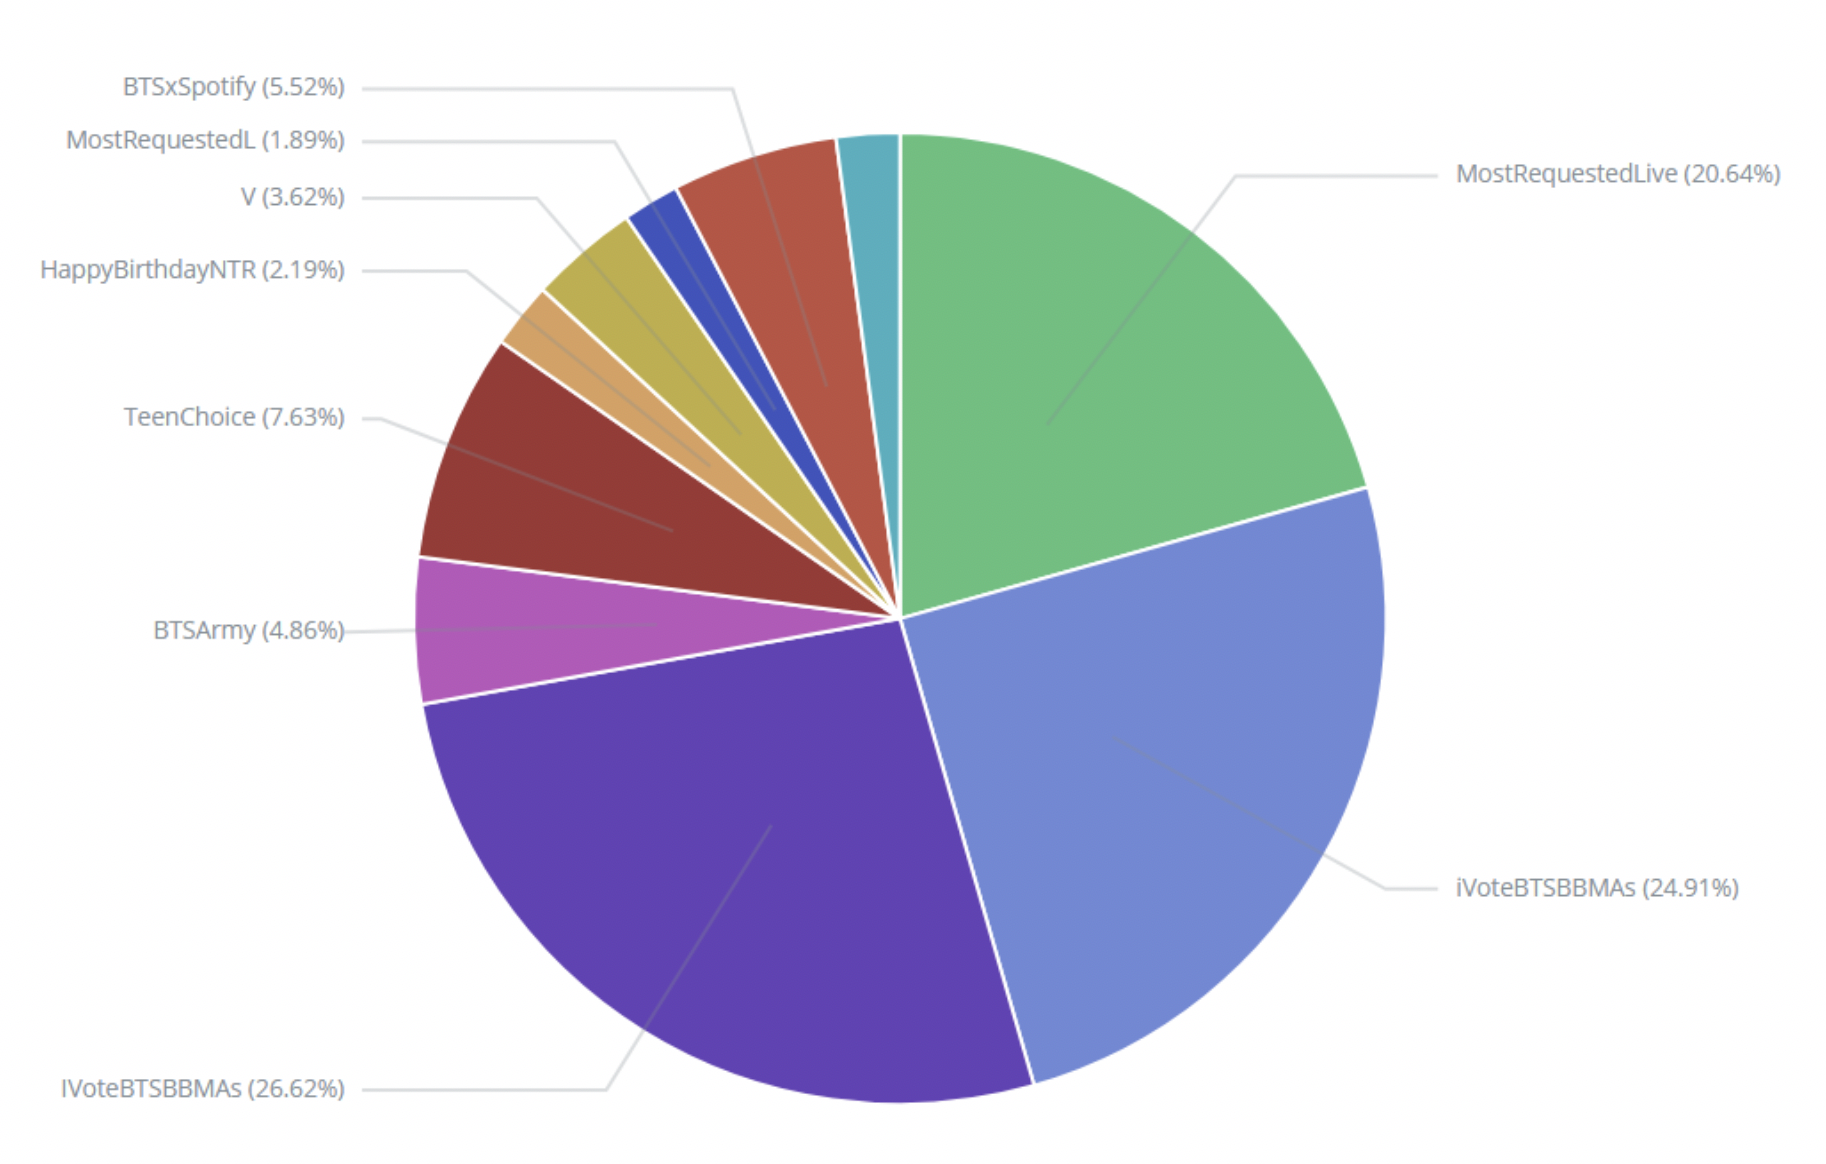
\includegraphics[scale=0.4]{material/architecture/kibana.png}
  \caption{Kibana Analyseplattform} 
  \label{fig:Kibana}
\end{figure}

\section{Fazit}
\subsection{Suchfunktionalität}
Jede moderne Software bietet eine Möglichkeit nach Daten zu suchen. Mit Hilfe von Elasticsearch kann eine einfache Suche nach einer Website oder einem Dokument innerhalb einer Sammlung implementiert werden. Anschließend kann eine Rechtschreibprüfung hinzugefügt werden. Höchstwahrscheinlich ist eine fuzzy Suche und automatische Vervollständigung nötig, möglicherweise sogar während der Eingabe. Da die Relevanz wichtig ist, können fortgeschrittene Ranking-Schemata erstellt werden. Zum Beispiel können Suchergebnisse basierend auf dem Standort, Zeit sowie des Benutzers ausgeführt werden. Und um zu wissen, was die Benutzer tatsächlich tun, kann die Nutzung der Software protokolliert und gespeichert werden für die spätere Analyse der Nutzerdaten.
\newline
Damit ist Elasticsearch eine moderne und mächtige Such-Engine, die fortgeschrittene Suchfunktionalität anbietet und für viele Anwendungsfälle geeignet ist.

\subsection{Performance}
Elasticsearch hat sich als eine robuste und fähige Such-Engine bewiesen, es konnte alle Ziele ohne Einschränkungen erfüllen und zusätzlich mit einer Vervollständigungsfunktion ergänzen. Die Index Konfiguration lässt sich einfach bedienen und über kleine Kalibrierungsschritte im JSON Format von einfachen bist komplexen Indexstrukturen erstellen. Von den Shards, Replicas bis zu den Data-Routings ist Cluster übergreifend alles möglich. Das Suchen ist eine etablierte IT-Disziplin, die mit Komfort, Kosten und Gewinn fest verbunden ist. Demgemäß ist Elasticsearch perfekt geeignet große Datenmengen zu durchsuchen und scheint mit der Anfragegeschwindigkeit, die mit jedem weiteren gefüllten Hardwareknoten die Anfragen automatisch parallelisiert. 
Somit bleibt die Geschwindigkeit im grünen Bereich auch nach dem Anstieg der Datenmenge.  
Allerdings haben die positiv gelisteten Eigenschaften ihre Tücken. Die Konfiguration des Indexes kann im Kleien so wie im Großen geschehen. Die richtige Hardware- (RAM/SSD/HDD) wie Indexkonfiguration muss gewissenhaft gewählt werden, um die versprochenen Geschwindigkeiten zu erreichen. Dementsprechend gewinnt man Zeit durch die automatisierte Datenverwaltung und verliert durch die Elasticsearch Wartung/Feinabstimmung. 

\subsection{Dokumentation und API}
Ebenso problematisch sind die Elasticsearch Abfragen, die einerseits gut im JSON-Format beschrieben und dokumentiert sind, jedoch in der Umsetzung, durch die von Elasticsearch zur Verfügung gestellten JAVA Bibliothek in JAVA schwer verständlich und Komplex in der Umsetzung.
Erst zum Ende des Projekts bin ich auf \textit{Mustach} gestoßen, die \terxtit{JSON-Templats} für die Abfragen erstellt und diese in einer simplen Form an Elasticsearch weiterleitet.  

\subsection{Tools}
Besondere positiv aufgefallen ist die WebUI Kibnan die mit Elasticsearch über REST Anfragen kommuniziert. Es ist möglich nach Daten zu suchen, den Clusterstatus abzufragen sowie aussagekräftige Grafiken zu erstellen. Diese Werkzeuge bieten dem Entwickler einen einfachen und übersichtlichen Einstig in die Elasticsearch-Umgebung. 

	%\chapter{Appendix D}

\section{Section 1}

\end{appendices}

% Esempio
%\index{Esempio |see{Esempio 2}}

\blankpage

%Indice analitico per il momento non verra' messo.
%\printindex %indice analitico


\bibliography{references}
\end{document}

%comandi utilizzati nel template:
%\texttt{} %per scrivere con carattere diverso
%\textbf{} %per scrivere con carattere diverso
%\href{http://www.blob.com/}{testo}
%\index{} %per indice analitico
%\footnote{} %note
%\noindent 
%\label{} 
%\ref{}
%\cite{PdfReference}
%\bibitem{PdfReference}
%®
%
%per inserire una figura:
%\begin{figure}[H]
%\begin{center}
%\includegraphics[width=12cm]{problematiche-del-ciclo-passivo.eps}\\
%\caption{Ciclo attivo e passivo in un'azienda}
%\label{fig:cicliAziendali}
%\end{center}
%\end{figure}
%
%per inserire una tabella:
%\begin{longtable}{p{3cm}p{9cm}}
%\textbf{Titolo} & Descrizione.\\
%\\
%\textbf{Titolo} & Descrizione.\\
%\\
%\end{longtable}
